%%%%%%%%%%%%%%%%%%%%%%%%%%%%%%%%%%%%%%%%%%%%%%%%%%%%%%%%%%%%%%%%%%%%%%%%%%%%%%%%
% Preámbulo                                                                    %
%%%%%%%%%%%%%%%%%%%%%%%%%%%%%%%%%%%%%%%%%%%%%%%%%%%%%%%%%%%%%%%%%%%%%%%%%%%%%%%%

\documentclass[11pt,a4paper,titlepage,oneside]{report}

%%% RELACIÓN DE VARIABLES A PERSONALIZAR %%%
%\def\lingua{gal}
\def\lingua{esp} % descomenta esta liña se redactarás a memoria en español
%\def\lingua{eng} % descomenta esta liña se redactarás a memoria en inglés
\def\nome{Abel González Vázquez}                             % substitúe aquí o teu nome
\def\nomedirectorA{Pablo Alejandro Calviño Padín}              % substitúe aquí o nome de quen dirixe


\def\titulo{Investigación sobre la eficiencia en la generación automática de código utilizando modelos de lenguaje masivos.} % substitúe aquí o título do teu TFG
\def\titulacion{gei}
\def\mencion{TECNOLOXÍAS DA INFORMACIÓN}

\def\renomearcadros{si} % descomenta esta liña se redactas a memoria en español e prefires que
                         % os "cuadros" e o "índice de cuadros" se renomeen
                         % a "tablas" e "índice de tablas" respectivamente

\usepackage{estilo_tfg}

% Lista de paquetes potencialmente interesantes (uso baixo demanda)


% \usepackage{alltt}       % proporciona o entorno alltt, semellante a verbatim pero que respecta comandos
% \usepackage{enumitem}    % permite personalizar os entornos de lista
% \usepackage{eurofont}    % proporciona o comando \euro
% \usepackage{float}       % permite máis opcións para controlar obxectos flotantes (táboas, figuras)
% \usepackage{hhline}      % permite personalizar as liñas horizontais en arrays e táboas
%  \usepackage{longtable}   % permite construir táboas que ocupan máis dunha páxina
% \usepackage{lscape}      % permite colocar partes do documento en orientación apaisada
% \usepackage{moreverb}    % permite personalizar o entorno verbatim
% \usepackage{multirow}    % permite crear celdas que ocupan varias filas da mesma táboa
% \usepackage{pdfpages}    % permite insertar ficheiros en PDF no documento
% \usepackage{rotating}    % permite diferentes tipos de rotacións para figuras e táboas
% \usepackage{subcaption}  % permite a inclusión de varias subfiguras nunha figura
% \usepackage{tabu}        % permite táboas flexibles
% \usepackage{tabularx}    % permite táboas con columnas de anchura determinada

%%%%%%%%%%%%%%%%%%%%%%%%%%%%%%%%%%%%%%%%%%%%%%%%%%%%%%%%%%%%%%%%%%%%%%%%%%%%%%%%
% Corpo                                                                        %
%%%%%%%%%%%%%%%%%%%%%%%%%%%%%%%%%%%%%%%%%%%%%%%%%%%%%%%%%%%%%%%%%%%%%%%%%%%%%%%%

\begin{document}

 %%%%%%%%%%%%%%%%%%%%%%%%%%%%%%%%%%%%%%%%
 % Preliminares do documento            %
 %%%%%%%%%%%%%%%%%%%%%%%%%%%%%%%%%%%%%%%%

 \begin{titlepage}
  
  \hspace*{128pt}
  \textcolor{udcpink}{{\fontencoding{T1}\fontfamily{phv}\selectfont Facultade de Informática}}\\[-32pt]

  \begin{center}
    
\includegraphics[scale=0.3]{imaxes/udc}\\[25pt]

    {\large TRABALLO FIN DE GRAO \\
            \nometitulacion \\
            \nomemencion } \\[10pt]

    \carimbo \\[25pt]

    \begin{huge}
      \begin{spacing}{1.3}
        \bfseries \titulo
      \end{spacing}
    \end{huge}
  \end{center}
  
  \vfill
  
  \begin{flushright}
    {\large
    \begin{tabular}{ll}
      {\bf Estudante:} & \nome \\
      {\bf Dirección:} & \nomedirectorA \\
%                      & \nomedirectorB \\ % duplica esta liña máis veces se o precisas, cambiando
                                           % a letra final (A, B, C, D...); define eses nomes no memoria_tfg.tex
    \end{tabular}}
  \end{flushright}
  \rightline{A Coruña, \datasimple.}
\end{titlepage}

 \dedicatoria{A mis abuelos} % escribe neste comando o teu texto de dedicatoria

\newpage % Esto crea una nueva página
\thispagestyle{empty} % Elimina encabezados y pies de página en esta página

\vspace*{\fill} % Añade espacio vertical antes del título para centrarlo verticalmente
\begin{center} % Comienza el entorno de centrado
\textbf{Agradecimientos} % Aplica negrita al título

\vspace{1em} % Añade un poco de espacio entre el título y el texto para separar visualmente

A mi familia, por su amor inquebrantable y su constante ánimo; a mis amigos, por su
compañerismo y motivación; y a mis profesores, por su guía experta y sus valiosos consejos.
Cada uno de ustedes ha sido fundamental para llevar a cabo este proyecto.
\end{center} % Cierra el entorno de centrado
\vspace*{\fill} % Añade espacio vertical después del texto para centrarlo verticalmente
\newpage % Opcional: Comienza una nueva página después de los agradecimientos si lo deseas


 %%%%%%%%%%%%%%%%%%%%%%%%%%%%%%%%%%%%%%%%%%%%%%%%%%%%%%%%%%%%%%%%%%%%%%%%%%%%%%%%

\pagestyle{empty}
\begin{abstract}
Los Modelos de Lenguaje Masivos son una importante innovación en inteligencia artificial, utilizando arquitecturas de redes neuronales profundas como los \textit{transformadores} para comprender y producir texto en lenguaje natural a gran escala. Algunos ejemplos notables son GPT y LLaMA.

Estos diseños han transformado la capacidad de las máquinas para comprender y crear texto coherente, junto con una amplia variedad de usos importantes, desde traducción automática hasta análisis de sentimientos y generación de texto. Su influencia alcanza a áreas como la investigación, la industria y la sociedad en su totalidad, generando nuevas oportunidades y retos en el terreno de la inteligencia artificial.

El propósito de esta iniciativa es aumentar la eficacia en la creación automática de código a través del empleo de estos grandes modelos de lenguaje. Exploraremos diversas tácticas para mejorar la precisión y la eficiencia en la producción automatizada de código, como el \textbf{Ajuste Fino} y la \textbf{Generación Aumentada de Recuperación.}

\vspace*{25pt}
\begin{segundoresumo}
Large Language Models are a significant innovation in artificial intelligence, utilizing deep neural network architectures such as \textit{transformers} to comprehend and produce text in natural language on a large scale. Some notable examples include GPT and LLaMA.

These designs have transformed the ability of machines to understand and generate coherent text, along with a wide variety of significant uses, from machine translation to sentiment analysis and text generation. Their influence extends to areas such as research, industry, and society as a whole, creating new opportunities and challenges in the field of artificial intelligence.

The purpose of this initiative is to enhance efficiency in automatic code generation through the use of these large language models. We are exploring various tactics to improve accuracy and efficiency in automated code production, such as \textbf{Fine-Tuning} and \textbf{Retrieval Augmented Generation}.
  \end{segundoresumo}
\vspace*{25pt}
\newpage  % Empieza una nueva página
\begin{multicols}{2}
\begin{description}
\item [\palabraschaveprincipal:] \mbox{} \\[-20pt]
\begin{itemize}
    \item Generación Automática de Código
    \item Modelos de Lenguaje Masivos
    \item Inteligencia Artificial
    \item Ajuste Fino
    \item Generación Aumentada de Recuperación 
    \item Transformadores
    \item Aprendizaje Profundo
    \item Eficiencia Computacional
    \item Ética en IA
\end{itemize}
\end{description}
\begin{description}
\item [\palabraschavesecundaria:] \mbox{} \\[-20pt]
\begin{itemize}
    \item Automatic Code Generation
    \item Large Language Models
    \item Artificial Intelligence
    \item Fine-Tuning
    \item Retrieval Augmented Generation
    \item Transformers
    \item Deep Learning
    \item Computational Efficiency
    \item AI Ethics
\end{itemize}
\end{description}
\end{multicols}

\end{abstract}
\pagestyle{fancy}

%%%%%%%%%%%%%%%%%%%%%%%%%%%%%%%%%%%%%%%%%%%%%%%%%%%%%%%%%%%%%%%%%%%%%%%%%%%%%%%%


 \pagenumbering{roman}
 \setcounter{page}{1}
 \bstctlcite{IEEEexample:BSTcontrol}


% Cambiar el nombre del pie de listado
\renewcommand{\lstlistingname}{Listado}

 \tableofcontents
 \listoffigures
 \listoftables
 \lstlistoflistings  % Índice de listados
 \clearpage
 
 \pagenumbering{arabic}
 \setcounter{page}{1}

 %%%%%%%%%%%%%%%%%%%%%%%%%%%%%%%%%%%%%%%%
 % Capítulos                            %
 %%%%%%%%%%%%%%%%%%%%%%%%%%%%%%%%%%%%%%%%
 \chapter{Introducción}
\label{chap:introduccion}

\section{Contexto y motivación}

\lettrine{E}{}n la actual sociedad digital, el desarrollo y actualización de software se ha convertido en una pieza clave en todos los ámbitos de nuestra vida diaria, abarcando desde aplicaciones móviles hasta sistemas críticos en diversas industrias. Sin embargo, el proceso de desarrollo de software es a menudo complejo y demandante, requiriendo habilidades especializadas y una considerable inversión de tiempo. Frente a este desafío, la generación automática de código emerge como una herramienta prometedora para mejorar la eficiencia y la productividad en la creación de software.

\bigskip % Deja una línea en blanco

La generación automática de código utiliza \acrlong{LLMs}, como \acrshort{GPT}, \acrshort{LLaMA} y Mixtral, que han sido entrenados con vastos conjuntos de datos de texto. Estos modelos han demostrado una capacidad impresionante para comprender y generar texto coherente y relevante, aplicado especialmente en la programación. No obstante, la precisión y eficacia del código producido por estos modelos son aspectos esenciales, ya que un código erróneo o ineficaz puede resultar en fallos críticos y brechas de seguridad. Aunque tiene sus ventajas, la amplia adopción de esta tecnología plantea cuestiones éticas y prácticas importantes, que van desde la equidad y accesibilidad en la programación hasta la seguridad e integridad del software creado.

\section{Objetivos de la investigación}

Este estudio se sumerge en la exploración de la generación automática de código utilizando los \acrfull{LLMs}, enfocándose en desentrañar y comprender las profundas implicaciones éticas y sociales que emergen de esta avanzada tecnología. El objetivo central de la investigación es realizar un \textbf{análisis crítico de las herramientas y sistemas actuales que facilitan la generación automática de código}, identificando tanto los desafíos como las oportunidades que ello representa. Además, se busca evaluar los riesgos potenciales asociados y proponer metodologías innovadoras que no solo mitiguen estos riesgos sino que también promuevan un desarrollo tecnológico ético y responsable.

\bigskip % Deja una línea en blanco

El enfoque se dirige hacia una exploración integral que incluye desde la \textbf{revisión de la literatura} existente hasta la \textbf{evaluación empírica} de diversas técnicas y enfoques. Esta investigación tiene la intención de ofrecer una perspectiva balanceada que considere tanto la eficiencia técnica como la responsabilidad social, apuntando hacia la creación de un marco de trabajo que guíe la implementación segura y ética de la generación automática de código en diferentes contextos industriales y sociales.

\bigskip % Deja una línea en blanco

Los propósitos principales de este trabajo es:

\begin{itemize}
\item Realizar una \textbf{revisión exhaustiva de la documentación} relevante sobre la generación automática de código y los modelos de lenguaje avanzados, incluyendo consideraciones éticas.
\item Compilar y \textbf{organizar conjuntos de datos} para el entrenamiento, asegurando diversidad y calidad, para evaluar la capacidad de estos modelos en la generación de código.
\item \textbf{Entrenar y evaluar varios \acrlong{LLMs} }utilizando métricas como precisión, recall y F1-score.
\item \textbf{Comparar diferentes enfoques}  de generación de código, como el uso de modelos preentrenados y técnicas de Fine-Tuning, para evaluar su efectividad, rapidez y adaptabilidad a diversos escenarios de programación.
\item Desarrollar \textbf{estándares éticos} para la utilización de la generación automática de código en el sector del software, con el fin de maximizar sus beneficios y minimizar los riesgos.
\end{itemize}

\bigskip % Deja una línea en blanco

\section{Estructura del trabajo}

A continuación, se muestra una breve síntesis de la estructura general de la memoria, resaltando los distintos capítulos y los temas que se abordarán en cada uno:

\begin{itemize}
    \item En el \Cref{chap:estadodelarte}, se analizarán los desarrollos recientes y los avances tecnológicos en la generación automática de código y en los modelos de lenguaje masivos. Además, se explorarán las herramientas más conocidas que actualmente facilitan la generación de código.
    
    \item En el \Cref{chap:conceptos}, se detallarán los principios teóricos que respaldan los modelos de lenguaje a gran escala. En este capítulo se abordará el tema de las estructuras de redes neuronales, como los transformadores, métodos de aprendizaje profundo, y enfoques de ajuste fino y generación aumentada de recuperación.
    
    \item En el \Cref{chap:planificacion}, se explorará la metodología utilizada en el estudio, que implica la elaboración del proyecto a través de un diagrama de Gantt y la organización de las tareas mediante un tablero Kanban. Se abordará la metodología Scrum de desarrollo ágil, mejorando la coordinación y control del avance. Por último, se llevará a cabo una evaluación de los gastos vinculados, especificando los elementos humanos y materiales requeridos para realizar el proyecto.
    
    \item En el \Cref{chap:tecnologías}, se detallarán las tecnologías clave utilizadas en el proyecto, incluyendo el \textit{hardware}, como el equipo informático, y el \textit{software}, como Visual Studio Code y Google Colab. Se mencionarán también las \acrshort{API}s esenciales como las de OpenAI y Hugging Face, destacando su papel en el entrenamiento y evaluación de modelos de lenguaje masivos.
    
    \item En el \Cref{chap:desarrollo}, se presentará la implementación práctica de los modelos y la configuración experimental utilizada. Se comentarán los resultados obtenidos de los experimentos, proporcionando análisis y comparaciones detalladas sobre la efectividad de diferentes modelos y configuraciones en la generación de código.
    
    \item En el \Cref{chap:etica}, se abordarán las consideraciones de seguridad, los dilemas éticos y el cumplimiento normativo relacionados con la generación automática de código. Además, se tratarán los estándares éticos y legales actuales y cómo estos afectan el diseño y la implementación de sistemas de generación de código.
    
    \item En el \Cref{chap:conclusions}, se resumirán las conclusiones y se brindarán recomendaciones para investigaciones venideras. Se planteará la posibilidad de seguir mejorando la generación automática de código mediante avances en modelos de lenguaje masivos, señalando posibles áreas de desarrollo futuro.
\end{itemize}



 \chapter{Estado del arte}
\label{chap:estadodelarte}

\lettrine{E}{}n el contexto actual del desarrollo de software, la incorporación de herramientas como \textbf{GitHub Copilot} y \textbf{OpenAI Codex} ofrecen la oportunidad de simplificar la creación de código con la asistencia de la inteligencia artificial. Estas herramientas se basan en modelos de lenguaje altamente experimentados, los cuales han sido entrenados con grandes volúmenes de datos de código. Este sistema no solo incrementa la eficacia al reducir las tareas repetitivas, sino que también promueve un enfoque más natural hacia la programación. En este capítulo se abordará el impacto y la implementación de estas modernas técnicas de programación en la industria del software.


\section{GitHub Copilot}

GitHub Copilot \cite{GitHubCopilot} (figura \ref{fig:1_MuestraCopilot}), desarrollado por GitHub tras su adquisición por Microsoft en 2018, representa una innovación significativa en la asistencia a la codificación mediante inteligencia artificial. Implementada a mediados de 2021, esta herramienta se integra en entornos de desarrollo como Visual Studio, Neovim o los \acrshort{IDE}s de JetBrains, dando lugar a sugerencias de código en tiempo real.

El origen de GitHub Copilot se basa en el modelo de lenguaje Codex de OpenAI, una versión especializada del conocido \acrshort{GPT}-3. Este modelo está diseñado para comprender y generar código en una variedad de lenguajes de programación, captando el contexto y la intencionalidad detrás de las entradas de los usuarios para ofrecer sugerencias pertinentes y funcionales.

Desde que se lanzó, más de 1.2 millones de desarrolladores han utilizado Copilot, resaltando su eficiencia en Python, con alrededor del 40 \% de sus sugerencias siendo usadas por los usuarios. Aunque puede crear nuevo código, la herramienta debe mejorar la precisión y relevancia de sus sugerencias para ser útil en entornos donde la exactitud es crucial.

\begin{figure}[htbp!]
  \centering
  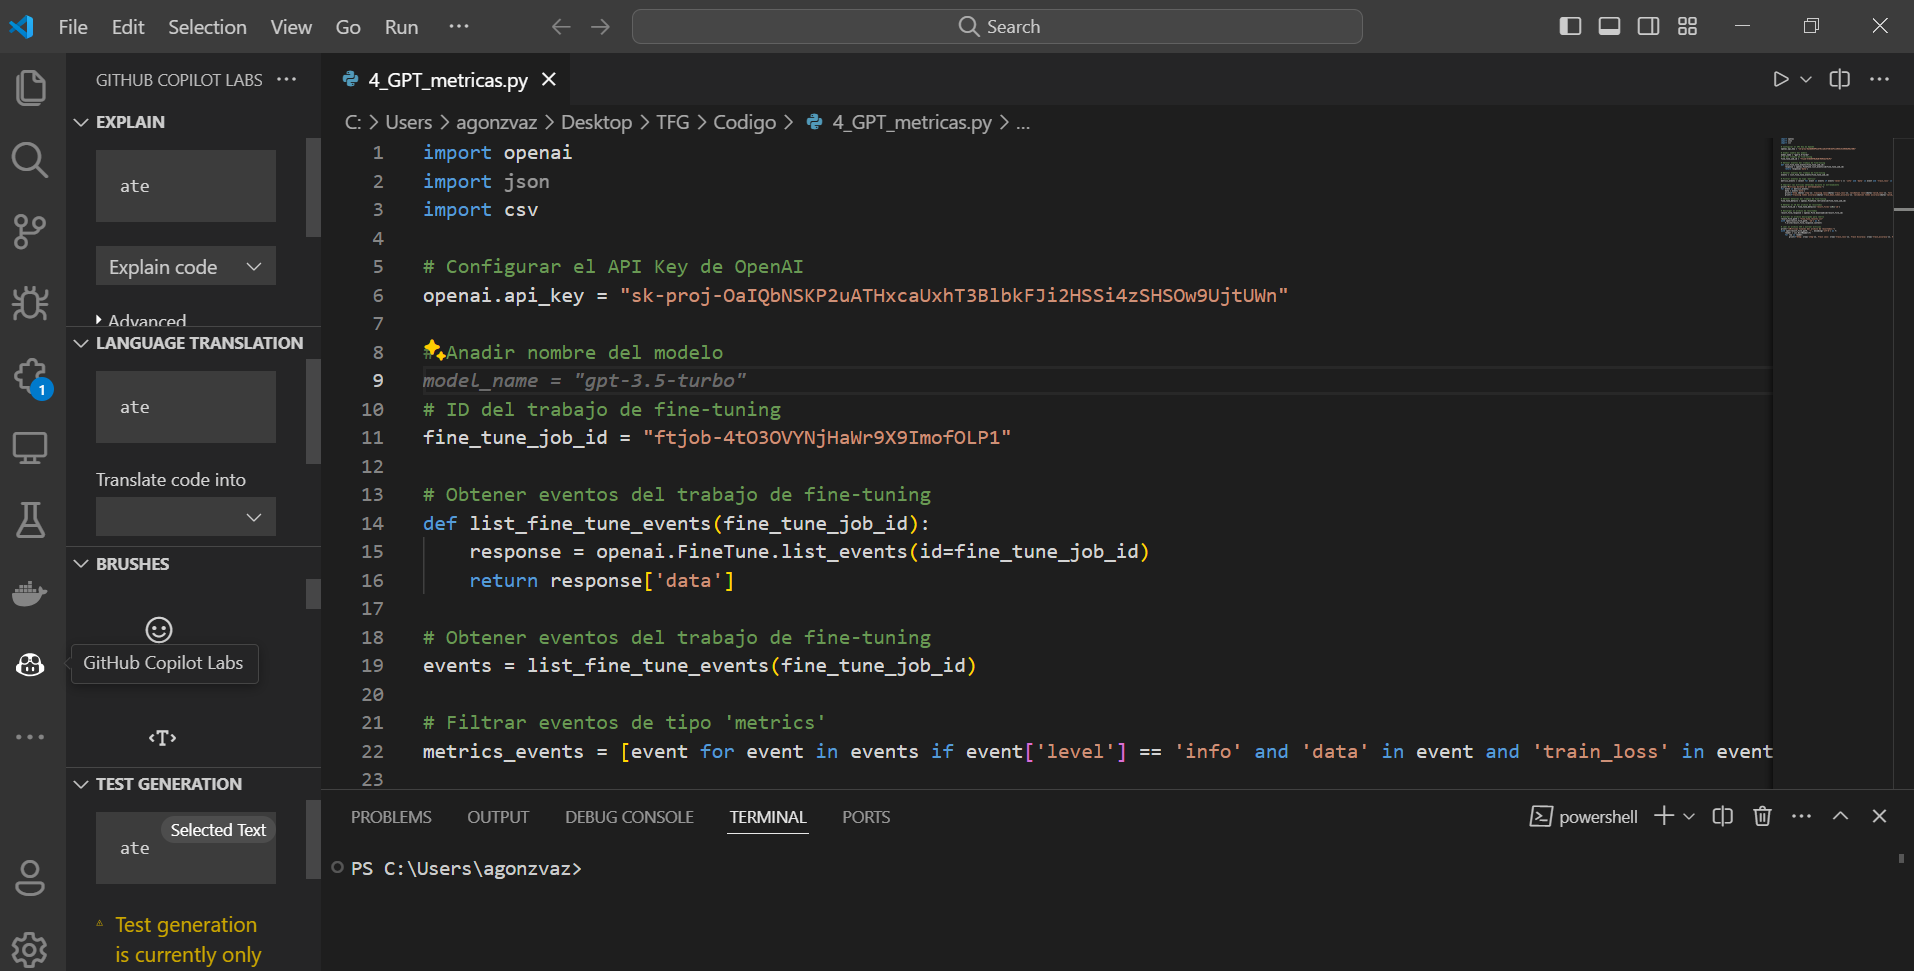
\includegraphics[width=1\textwidth]{imaxes/1_MuestraCopilot.png}
\caption{Ejemplo práctico del funcionamiento de GitHub Copilot.}
  \label{fig:1_MuestraCopilot}
\end{figure}


\section{OpenAI Codex}

OpenAI Codex \cite{OpenAICodex}, desarrollado por OpenAI, es una herramienta que interpreta el lenguaje natural y genera código. Codex, basado en el exitoso GitHub Copilot, es un producto generado a partir del modelo \acrshort{GPT}-3 de OpenAI, creado específicamente para emplearse en tareas de programación. Su lanzamiento en una fase beta exclusiva ha sido respaldado por una extensa capacitación en 159 GB de código Python extraído de 54 millones de repositorios en GitHub.

Codex hace más fácil escribir código al ofrecer sugerencias específicas y adecuadas, y también puede comprender y seguir instrucciones en lenguaje natural. Gracias a su capacidad para aprender varios lenguajes de programación, es capaz de participar en diferentes proyectos de desarrollo de software. La \acrshort{API} exclusiva de Codex permite cambiar la forma en que los desarrolladores interactúan con el software al integrar funciones de generación de código, acelerando la creación y fomentando la innovación en programación.
 \chapter{Conceptos teóricos}
\label{chap:conceptos}


\lettrine{E}{}n este capítulo se abordan los conceptos fundamentales necesarios para la realización de este \acrfull{TFG}.

\section{Modelos de lenguaje masivos}

Los \acrfull{LLMs} son un tipo de modelos de inteligencia artificial que utiliza técnicas de aprendizaje automático para comprender y producir lenguaje humano. Estas herramientas pueden ser de gran utilidad para las compañías y organizaciones que desean automatizar y mejorar diferentes áreas de la comunicación y del análisis de datos.

Los \acrshort{LLMs} utilizan modelos basados en redes neuronales y técnicas de \acrfull{NLP} para procesar y estimar sus resultados. El \acrshort{NLP} es un campo de la inteligencia artificial que se centra en lograr que las computadoras comprendan, interpreten y generen texto. Esto, a su vez, permite que los \acrshort{LLMs} realicen diversas tareas: analizar texto y sentimientos u opiniones, traducir idiomas y reconocer voces.

Los \acrshort{LLMs}, como \acrfull{GPT} y \acrfull{LLaMA}, utilizan un método conocido como aprendizaje no supervisado para comprender y procesar el lenguaje natural. En este proceso, se proporcionan extensos conjuntos de datos al modelo, que los analiza y aprende de forma autónoma a través de ejemplos sin etiquetar previamente. Esta fase de preentrenamiento es crucial para desarrollar la capacidad del modelo de generar respuestas coherentes y contextualmente adecuadas sin supervisión directa.

Debido a la necesidad de realizar cálculos constantes de probabilidades para encontrar conexiones, \acrshort{LLMs} requieren una cantidad significativa de recursos computacionales. Las \acrfull{GPU}s son uno de los recursos utilizados para obtener potencia informática. Las \acrshort{GPU}s son dispositivos  especializados de hardware diseñados para gestionar tareas complejas de procesamiento paralelo, lo que hace que sean ideales para los modelos de aprendizaje automático y aprendizaje profundo que requieren realizar numerosos cálculos.

\subsection{Aprendizaje Profundo}

La técnica de inteligencia artificial conocida como aprendizaje profundo consiste en enseñar a las computadoras a procesar datos utilizando algoritmos que se inspiran en el cerebro humano. Este método, denominado aprendizaje profundo o redes neuronales profundas \cite{IBM}, posibilita que las computadoras aprendan mediante la observación, similar a los seres humanos.

Las \acrfull{ANN} son la base del aprendizaje profundo y se basan en el funcionamiento de las neuronas biológicas, pero utilizan neuronas artificiales formadas por nodos de software, como se muestra en la figura \ref{fig:2_Deep Neuronal Network}. Los nodos se valen de operaciones matemáticas (en vez de procesos químicos como el cerebro) para intercambiar y transferir datos en el sistema.

\begin{figure}[hp!]
  \centering
  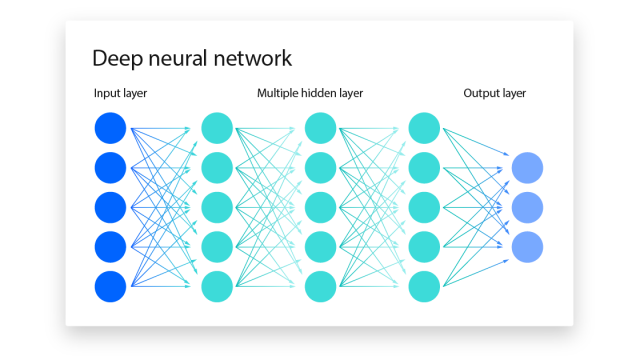
\includegraphics[width=0.75\textwidth]{imaxes/2_Deep Neuronal Network.png}
\caption[Esquema de una Red Neuronal Profunda]{Esquema de una Red Neuronal Profunda. \textit{Fuente: \cite{ResearchGate2024}}}
  \label{fig:2_Deep Neuronal Network}
\end{figure}

\subsection{IA Generativa}
\label{subsec:iagenerativa}


La inteligencia artificial generativa (\acrshort{GenAI}) \cite{IAGenerativa} representa una faceta de la inteligencia artificial que se especializa en la creación de nuevo contenido a través de modelos de aprendizaje profundo. Estos modelos son diferenciados por su habilidad de producir \textbf{ información innovadora} y \textbf{única}, en contraste con los modelos de IA discriminativa, los cuales se centran en la clasificación o distinción entre datos ya existentes. La inteligencia artificial generativa se aprovecha de grandes bases de datos para devolver salidas de calidad, las cuales son creaciones originales que imitan las características de los datos iniciales.

La versatilidad de la \acrshort{GenAI} se demuestra en sus diferentes usos, como la creación de textos, imágenes, y código de software, además de su aplicación en la investigación científica. ChatGPT, DALL-E, GitHub CoPilot \ref{chap:estadodelarte} son algunos de los ejemplos más reconocidos de la \acrlong{GenAI}.
Estos modelos funcionan a través de algoritmos de aprendizaje profundo que generan representaciones codificadas de los datos en los que fueron entrenados, siendo estas representaciones simplificaciones que posibilitan la creación de nueva información manteniendo la esencia de los datos originales. El procedimiento incluye la utilización de métodos como el refinamiento supervisado y la optimización específica para cada situación, garantizando que el resultado sea adecuado para el usuario.

Aunque tiene beneficios, la \acrlong{GenAI} presenta importantes desafíos, especialmente en el ámbito ético y de la seguridad. Contar con la habilidad de crear contenido realista puede resultar en la producción de información falsa o contenido inadecuado, por lo que se necesita un fuerte marco ético y medidas de seguridad sólidas para reducir estos peligros.

\subsubsection{Transformers}
\label{subsubsec:transformers}

Los Transformers son una variedad de \acrfull{DNN} que resuelven los problemas de las arquitecturas secuencia a secuencia, como la dependencia corta de las secuencias de entrada y el procesamiento secuencial, lo que dificulta el entrenamiento en paralelo. Los transformadores \cite{bender2022generacion} utilizan el mecanismo de \textbf{autoatención de múltiples cabezales} para extraer atributos y tienen un alto potencial para usarse en \acrshort{NLP}. En contraste con las técnicas convencionales de recurrencia, Transformers emplean la atención para entender todo un fragmento de una secuencia, mediante bloques de codificación y decodificación, como podemos observar en la figura \ref{fig:2_Transformer}.

La habilidad de Transformers para capturar el verdadero significado del contexto es una ventaja fundamental sobre \acrfull{LSTM} y  \acrfull{RNN}, gracias a su mecanismo de atención. Igualmente, los Transformers son veloces porque tienen la capacidad de operar simultáneamente, a diferencia de las redes recurrentes, y son capaces de aprovechar \acrshort{GPU}, lo que resulta en una ejecución más rápida de tareas que tienen entradas extensas. Los beneficios del modelo Transformer han motivado a expertos del aprendizaje profundo a investigar su utilidad en distintas áreas y ha generado numerosas publicaciones y la creación de modelos basados en Transformer para diversas funciones en inteligencia artificial.

\begin{figure}[!htb]
  \centering
  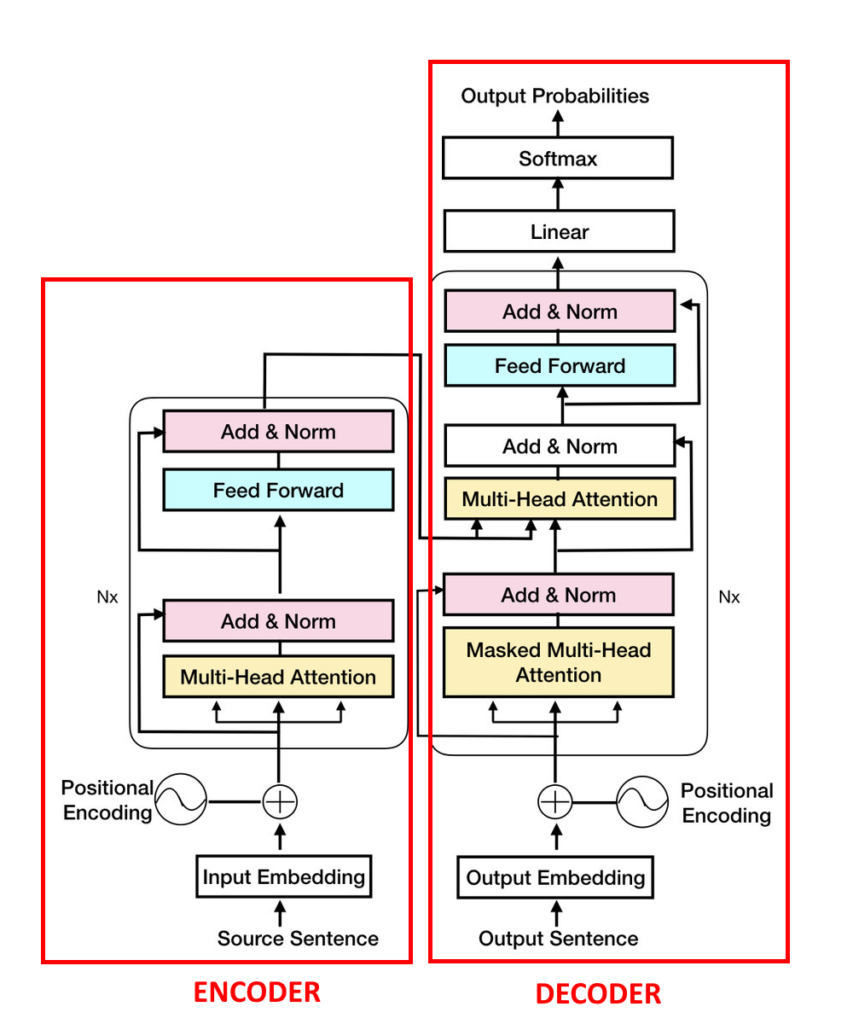
\includegraphics[width=0.60\textwidth]{imaxes/2_Transformer.png}
  \caption[La Arquitectura de los Transformers]{La Arquitectura de los Transformers. \textit{Fuente: \cite{vaswani2023attention}}}
  \label{fig:2_Transformer}
\end{figure}


\newpage
\subsubsection{Enfoque de Fine-Tuning}
\label{subsubsec:enfoquefinetuning}

Fine-Tuning, también conocido como Ajuste Fino \cite{IBM_Fine}, es una práctica frecuente en el ámbito del aprendizaje automático, especialmente en el \acrshort{NLP}. Dentro del contexto de los \acrshort{LLMs}, como \acrshort{GPT}-3 o \acrshort{LLaMA}, este enfoque consiste en modificar los parámetros de un modelo previamente entrenado con una gran cantidad de datos, utilizando información específica de la tarea a resolver.

Por lo tanto, consiste en volver a entrenar únicamente algunas secciones del modelo, por lo general las capas finales o algunas capas específicas, dejando las capas iniciales sin cambios. Esto posibilita que el modelo preentrenado mantenga el conocimiento general adquirido en el preentrenamiento inicial, mientras se ajusta a la tarea específica para la cual está siendo adaptado.

En el caso de la generación automática de código, se podría usar un modelo de lenguaje grande preentrenado, como \acrshort{GPT}-3, y modificarlo con un conjunto de datos específico de ejemplos de código y descripciones en lenguaje natural. El modelo se entrenará para producir código con mayor precisión y coherencia, adaptándose a las especificaciones dadas.

\subsubsection{Enfoque RAG}
\label{subsubsec:enfoquerag}

El \acrfull{RAG} es una técnica que complementa la generación de texto con información de fuentes de datos privadas o propietarias\cite{GobiernoEspana_RAG}. Combina un modelo de recuperación, que está diseñado para buscar grandes \textit{sets} de datos o bases de conocimiento, con un modelo de generación como el \acrfull{LLMs}, que toma esa información y genera una respuesta de texto legible como se muestra en la figura \ref{fig:2_RAG}.

Incrementar la generación de recuperación puede elevar la importancia de una búsqueda al incluir información extra y complementar el conocimiento inicial del entrenamiento de un \acrshort{LLMs}. Esto aumenta la eficacia del gran modelo de lenguaje sin la necesidad de reentrenarlo. Las fuentes de información extra pueden incluir desde datos nuevos en línea no adiestrados por el \acrshort{LLMs} hasta información confidencial interna de compañías o contexto comercial exclusivo.

\bigskip % Deja una línea en blanco

\begin{figure}[hp!]
  \centering
  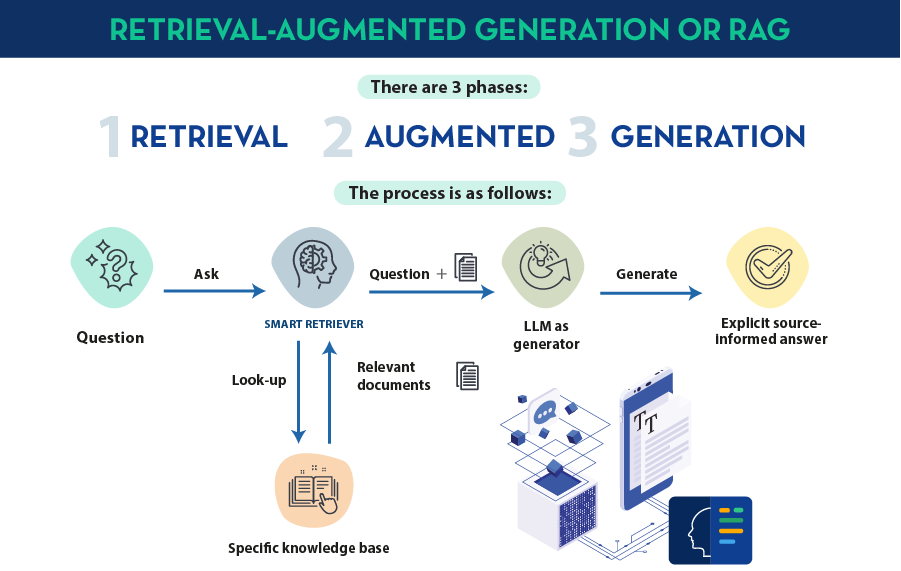
\includegraphics[width=0.75\textwidth]{imaxes/2_RAG.png}
  \caption[Esquema del funcionamiento de un Modelo RAG]{Esquema del funcionamiento de un Modelo RAG. \textit{Fuente: \cite{GobiernoEspana_RAG}}}
  \label{fig:2_RAG}
\end{figure}




 \chapter{Planificación}
\label{chap:planificacion}

\lettrine{E}{}n este capítulo se presentan las metodologías de desarrollo elegidas para la realización del proyecto, así como los costes y la organización temporal.

\section{Metodología de desarrollo}

Se seleccionó \textbf{Scrum} \cite{sachdeva2016scrum} como la metodología para este proyecto. Es un enfoque ágil para el desarrollo de software que tiene como objetivo administrar proyectos con flexibilidad y enfocándose en maximizar el retorno de la inversión (ROI). Scrum fue creado alrededor de 1986 por \textbf{Ikujiro Nonaka e Hirotaka Takeuchi}, inspirado en una investigación hecha en varias compañías que estaban implementando un enfoque laboral innovador. Este marco de referencia establece un grupo de eventos, prácticas y roles, y puede ser utilizado como punto de inicio para definir el procedimiento de producción que un equipo de trabajo empleará en un proyecto.


Los principios de Scrum se centran en:

\begin{itemize}
\item \textbf{Control empírico de procesos:} Se basa en la transparencia, inspección y adaptación para aprender a través de la experimentación, especialmente en situaciones donde el problema no está claro.
\item \textbf{Autoorganización:}  Los equipos logran un mayor valor cuando se autoorganizan, lo que fomenta una mejor participación, responsabilidad compartida y un entorno creativo propicio para el crecimiento. 
\item \textbf{Colaboración:} Destaca la importancia de la conciencia, articulación y apropiación en el trabajo colaborativo, involucrando a equipos, clientes y partes interesadas para crear valor compartido.
\item \textbf{ Priorización basada en valores:} Se enfoca en ofrecer el máximo valor comercial desde el principio hasta el final del proyecto.
\item \textbf{Timeboxing:} El tiempo se considera una restricción importante en Scrum y se utiliza para gestionar eficazmente la planificación y ejecución del proyecto.
\item \textbf{Desarrollo iterativo:} Se centra en gestionar cambios y crear productos que satisfagan las necesidades del cliente, delineando las responsabilidades del propietario del producto y la organización en el desarrollo iterativo.
\end{itemize}

\begin{figure}[hp!]
  \centering
  \includegraphics[width=0.75\textwidth]{imaxes/3_SCRUM.png}
  \caption[Marco de trabajo SCRUM]{Marco de trabajo SCRUM. \textit{Fuente: \cite{AusumScrum2024}}}
  \label{fig:3_SCRUM}
\end{figure}


\section{Planificación del proyecto}

Para planificar el desarrollo del proyecto, se utilizó un \textbf{diagrama de Gantt} \cite{diagramaGantt}. Este gráfico ofrece un cronograma del proyecto donde se pueden visualizar las fechas de inicio y finalización de las tareas y hitos. Cada tarea se representa con una barra horizontal que indica su duración, con fechas de inicio y finalización acordadas antes del inicio del proyecto.

En la siguiente figura \ref{fig:3_DiagramaGantt}, se muestra el inicio y la finalización del proyecto. La finalización está programada una semana antes de la entrega para permitir una revisión exhaustiva.

Es importante destacar que se llevan a cabo reuniones semanales con el tutor para realizar un seguimiento del progreso del proyecto.

Se ha implementado la metodología Scrum en el desarrollo del proyecto. Durante la organización de este proyecto se seguirán las siguientes etapas distintivas:
\begin{itemize}
\item \textbf{Sprint Planning:} En este comienzo de Scrum se trata de detallar las responsabilidades de los integrantes del equipo y estimar el tiempo para completarlas.
\item \textbf{Scrum Team Meeting:}  Reuniones informativas y diarias realizadas por los equipos laborales para revisar avances, analizar tareas del día y solucionar problemas actuales o potenciales.
\item \textbf{Backlog Refinement:} Implica que el \acrfull{PO} (tutor) revise las tareas y su avance para evaluar el tiempo y esfuerzo dedicados a cada tarea y solucionar cualquier problema que surja durante el proceso.
\item \textbf{Sprint Review:} Se trata de una reunión donde el cliente (tutor) está presente y se enfoca en presentar los logros alcanzados durante el sprint.
\item \textbf{Retrospective:} Este encuentro final se realiza al terminar el proyecto y se centra en analizar todo lo sucedido durante el mismo, con el fin de obtener aprendizajes para mejorar en próximos proyectos.
\end{itemize}

\begin{figure}[h]
  \centering
  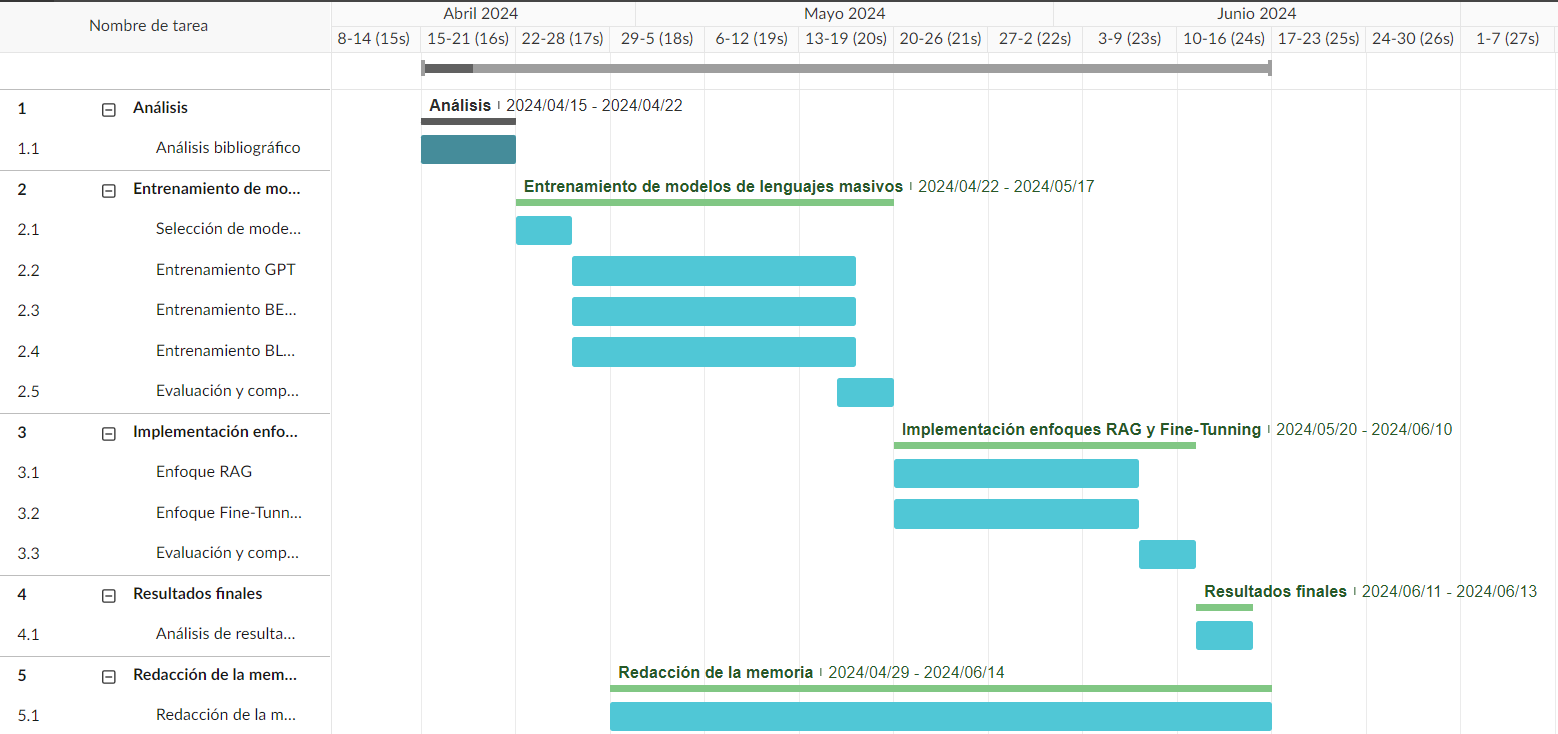
\includegraphics[width=\linewidth,height=\textheight,keepaspectratio]{imaxes/3_DiagramaGantt.png}
  \caption{Diagrama de Gantt del proyecto.}
  \label{fig:3_DiagramaGantt}
\end{figure}


\subsection{Fases}

La primera fase, \textbf{Análisis}, contiene 1 tarea:
\begin{itemize}
    \item \textbf{Tarea 1.1: Análisis bibliográfico.} En esta tarea se recopiló la información fundamental para iniciar el desarrollo del proyecto, incluyendo las tecnologías empleadas, la comprensión del dominio del problema, entre otros aspectos relevantes. Duración 1 semana y esfuerzo 40h.
\end{itemize}

La siguiente fase es \textbf{Entrenamiento de modelos de lenguajes masivos}, contiene 5 tareas:
\begin{itemize}
    \item \textbf{Tarea 2.1: Selección de modelos y conjunto de datos.} Implica elegir los modelos más apropiados y un conjunto de datos adecuado que nos facilite la realización de pruebas de manera óptima. Duración 3 días y esfuerzo 24h.
    \item \textbf{Tarea 2.2: Entrenamiento \acrshort{GPT}.} Entrenar el modelo \acrshort{GPT} utilizando el conjunto de datos seleccionado con el fin de obtener resultados satisfactorios y aprovechar al máximo la capacidad de este modelo de lenguaje masivo.
    Duración 2 semanas y esfuerzo 20h.
    \item \textbf{Tarea 2.3: Entrenamiento \acrshort{LLaMA}.} Entrenar el modelo \acrshort{LLaMA} utilizando el conjunto de datos seleccionado con el fin de obtener resultados satisfactorios y aprovechar al máximo la capacidad de este modelo de lenguaje masivo.
    Duración 2 semanas y esfuerzo 20h.
    \item \textbf{Tarea 2.4: Entrenamiento Mixtral.} Entrenar el modelo Mixtral utilizando el conjunto de datos seleccionado con el fin de obtener resultados satisfactorios y aprovechar al máximo la capacidad de este modelo de lenguaje masivo.
    Duración 2 semanas y esfuerzo 20h.
    \item \textbf{Tarea 2.5: Evaluación y comparativa de resultados.} Analizar y evaluar los resultados obtenidos por los diferentes modelos.
    Duración 3 días y esfuerzo 18h.
\end{itemize}

La siguiente fase, \textbf{Implementación de los enfoques \acrshort{RAG} y Fine-Tuning}, tiene 3 tareas:
\begin{itemize}
    \item \textbf{Tarea 3.1: Implementación enfoque \acrshort{RAG}.} Implementación del enfoque RAG en el proyecto, configurando y desarrollando el modelo de generación de código utilizando \acrfull{RAG} como base, con ajustes y personalizaciones para adaptarse a los requisitos del proyecto. Duración 1'5 semanas y esfuerzo 22'5h.
    \item \textbf{Tarea 3.2: Implementación enfoque Fine-Tuning.}
     Ajustar un modelo de lenguaje preentrenado para que se especialice en generar código, adaptándolo específicamente para las necesidades de este proyecto con el enfoque Fine-Tuning. Duración 1'5 semanas y esfuerzo 22'5h.
     \item \textbf{Tarea 3.3: Evaluación y comparativa de resultados.} Analizar los resultados obtenidos y las conclusiones relacionadas con la eficacia de cada enfoque utilizado en el proyecto. Duración 3 días y esfuerzo 15h.
\end{itemize}

La siguiente fase, \textbf{Resultados finales}, tuvo una sóla tarea:
\begin{itemize}
    \item \textbf{Tarea 4.1: Análisis de resultados finales.} Analizar los resultados obtenidos en todo el proyecto y obtener las conclusiones del proyecto. Duración 3 días y esfuerzo 15h.
\end{itemize}

Finalmente, tenemos la fase \textbf{Redacción de la memoria}, con una única tarea:
\begin{itemize}
    \item \textbf{Tarea 5.1: Redacción de la memoria.} Actividad llevada a cabo durante todo el proyecto para mantener actualizada la memoria con los avances realizados. Duración 3'5 semanas y esfuerzo 35h.
\end{itemize}

\section{Tablero Kanban}
Para obtener una visión más clara del progreso del proyecto, se ha optado por utilizar un \textbf{tablero Kanban} \cite{tableroKanban} para el seguimiento y la realización de las tareas. En la figura \ref{fig:3_TableroKanban}  se pueden observar todas las tareas por realizar y su estado actual. Una ventaja de utilizar este tablero es su integración con el Diagrama de Gantt, de modo que cualquier cambio en la estimación del tiempo de una tarea se reflejará automáticamente en el otro.

\begin{figure}[h]
  \centering 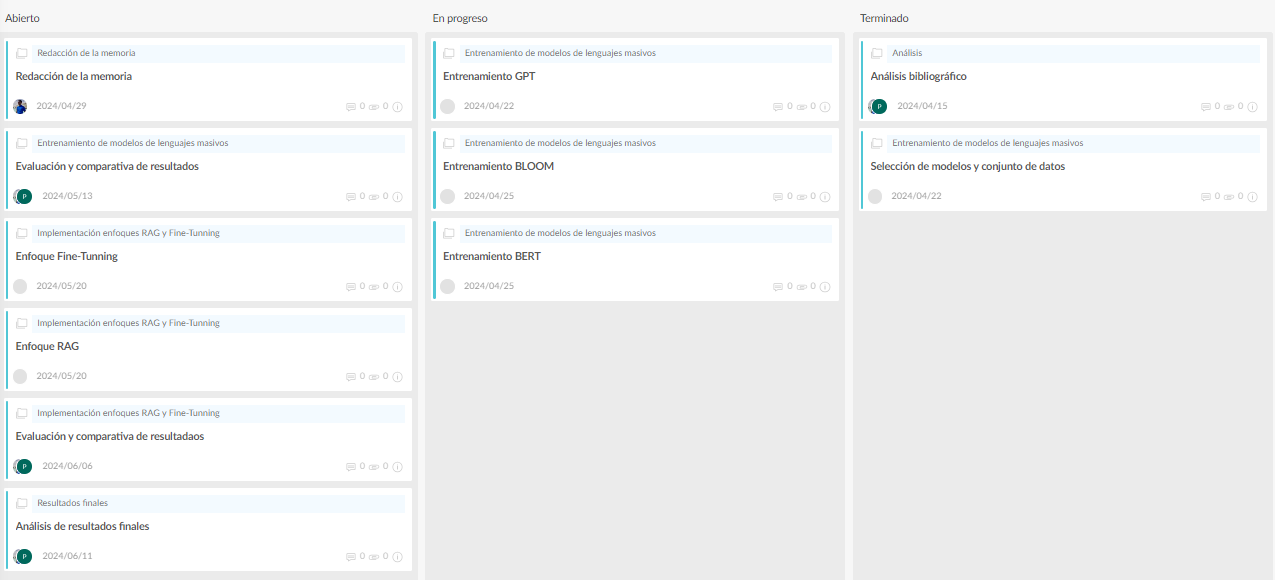
\includegraphics[width=\linewidth,height=\textheight,keepaspectratio]{imaxes/3_TableroKanban.png}
  \caption{Tablero Kanban del proyecto en desarrollo.}
  \label{fig:3_TableroKanban}
\end{figure}

\section{Estimación de costes}
Al calcular el coste del proyecto, se consideraron el tiempo dedicado, los recursos humanos necesarios y los materiales utilizados.

\subsection{Recursos humanos}
Al calcular el costo del proyecto, se parte del supuesto de que se lleva a cabo a tiempo completo, sin interrupciones, lo que equivale a una jornada de 40 horas semanales o 160 horas mensuales. Por lo tanto, considerando una duración total del proyecto de 360 horas y una semana laboral de 40 horas, se estima una duración de 9 semanas.

Para un desarrollador junior con un sueldo por hora de 11€, el costo total del trabajo sería de \textbf{3960€}.

Por otro lado, el tutor que desempeña la función de \acrfull{PO} tiene un sueldo de 30€ por hora. Dado que el proyecto se extiende a lo largo de 9 semanas y se realizan reuniones semanales de 1 hora, con una revisión final adicional de 10 horas, el costo total del \acrshort{PO} sería de \textbf{570€}.

\subsection{Recursos materiales}

La gran mayoría del software utilizado es software libre, por lo que no hemos tenido que pagar licencias para su uso. En el caso del software privativo, se han utilizado versiones gratuitas, excepto en el caso del \acrshort{API} de OpenAI \cite{APIOpenApi}, donde el costo depende del número de \gls{token}s utilizados y se estima en \textbf{20€}.

En cuanto al equipo informático, no se ha agregado ningún costo, ya que los equipos ya están completamente amortizados.

Por otro lado, en cuanto a los gastos de electricidad e internet, la electricidad representa un costo de \textbf{80€} por aproximadamente 3 meses de trabajo, mientras que el acceso a internet supone un costo de 23€ al mes, es decir, \textbf{69€} en total.


\subsection{Coste total}

En la siguiente tabla ~\ref{tab:Coste total proyecto}  se realiza un desglose del costo total del proyecto.

\begin{table}[hp!]
  \centering
  \rowcolors{2}{white}{udcgray!25}
  \begin{tabular}{c|c}
  \rowcolor{udcpink!25}
  \textbf{Concepto} & \textbf{Coste} \\\hline
  \textit{Desarrollador junior} & 3960€ \\
  \textit{\acrlong{PO}} & 570€ \\
  \textit{\acrshort{API} de OpenAI} & 20€ \\
  \textit{Electricidad} & 80€ \\
  \textit{Internet} & 69€ \\
  \textit{\textbf{COSTE TOTAL}} & \textbf{4699€} \\
  \end{tabular}
  \caption{Tabla con el desglose del coste total.}
  \label{tab:Coste total proyecto}
\end{table}
 \chapter{Tecnologías utilizadas}
\label{chap:tecnologías}

\lettrine{E}{}n este capítulo se describen las tecnologías empleadas para la realización del \acrshort{TFG}, tanto el equipo informático como el software.


\section{Equipo informático}
\label{sec:mostra}

El proyecto se ha realizado con un portátil Dell Latitude 5410 con las siguientes características:

\begin{itemize}
    \item \acrfull{CPU}: Intel(R) Core(TM) i5-10310U CPU @ 1.70GHz, 2208 Mhz
    \item \acrfull{GPU}: Intel(R) UHD Graphics con 7992 MB de memoria DDR4
    \item \acrfull{RAM} 16GB de memoria DDR4
    \item Almacenamiento: PM991 NVMe Samsung 256GB de memoria \acrfull{SSD}
    \item \acrfull{SO}: Windows 10 Enterprise
\end{itemize}

\section{Software}
\label{sec:mostra}

\begin{itemize}
    \item El editor de código fuente elegido ha sido \textbf{Visual Studio Code} \cite{VSC}. Es un editor de código fuente desarrollado por Microsoft, disponible de manera gratuita y con código abierto.
    \item Hemos empleado como entorno virtual \textbf{Google Colab} \cite{GoogleColab}. Es un servicio alojado de Jupyter Notebook que no requiere configuración y que ofrece acceso gratuito a recursos de computación, como GPUs y TPUs.
    \item El lenguaje de programación elegido ha sido \textbf{Python 3.11.5} \cite{Python}, siendo este un lenguaje de programación interpretado, orientado a objetos, de alto nivel y con semántica dinámica.
    \item Para el manejo de ficheros parquet hemos empleado la herramienta \textbf{ParquetViewer}  para trabajar con archivos parquet \cite{GobiernoEspana_Parquet} debido a su facilidad y rapidez en la manipulación de dichos archivos. Esto ocurre debido al almacenamiento de datos en formato columnar, lo que permite la compresión y la eliminación de datos duplicados. Mejorando de esta manera el desempeño en la escritura y lectura, además de la capacidad de análisis.
    \item Como herramienta para probar los \acrlong{LLMs} entrenados hemos usado \textbf{LM Studio} \cite{LMStudio}.
    \item \textbf{Chroma DB} \cite{Chroma} es una base de datos vectorial de código abierto diseñada específicamente para aplicaciones con los \acrfull{LLMs}.
    \item Como conjunto de datos hemos optado por \textbf{The Vault} \cite{TheVault}. Es un \textit{dataset} con diferentes problemas de programación y sus posibles soluciones en diferentes lenguajes, en nuestro caso solamente usaremos aquellos realizados en Python.
    \item Hemos empleado diferentes \acrshort{API}s para tener acceso a los diferentes modelos, como fueron las de \textbf{OpenAI} \cite{APIOpenApi}y \textbf{Hugging Face} \cite{HuggingFace}, la cual es una plataforma que proporciona modelos preentrenados y herramientas para el \acrlong{NLP}, facilitando el acceso y la implementación de tecnologías avanzadas de \acrshort{AI}. Además, para trabajar con \textit{embeddings}, utilizamos el \acrshort{API} de \textbf{Nomic} \cite{Nomic}, especializado en su creación, visualización, y análisis de datos.    
    \item Para la instalación de las siguientes librerías hemos utilizado \textbf{pip 24.0} \cite{Pip}.
    \item Librerías utilizadas para acceder a funcionalidades de los modelos usados: \textbf{openAi} \cite{APIOpenApi} y \textbf{hugginsface\_hub} \cite{HuggingFace}.
    \item \textbf{Transformers} \cite{Transformers} es una librería que proporciona APIs para descargar y entrenar fácilmente modelos preentrenados de última generación, y la librería \textbf{datasets} [REF] para la carga y manipulación de datos.
    \item Como herramienta para realizar entrenamiento en el modelo usamos la librería \textbf{tlr} \cite{Tlr} y \textbf{torch} \cite{Torch}, que forma parte de la biblioteca PyTorch. Es un framework de aprendizaje profundo que facilita tanto la construcción como el entrenamiento de modelos.
    \item La librería \textbf{peft} \cite{Peft} está diseñada para la adaptación eficiente de modelos preentrenados a aplicaciones específicas sin necesidad de ajustar todos los parámetros del modelo.
    \item Para el apartado de métricas hemos usado las librerías \textbf{nltk} \cite{Nltk}y \textbf{sklearn.metrics} \cite{SklearnMetrics}.
    \item Para visualizar el entrenamiento de modelos de aprendizaje automático, hemos empleado \textbf{TensorBoard} \cite{TensorBoard} integrada en TensorFlow.
    \item Para la realización de la memoria se usó \textbf{Overleaf} \cite{Overleaf}, una herramienta en línea para la edición de documentos en LaTeX.
    \item Finalmente, hemos utilizado \textbf{GitHub} como repositorio para alojar el conjunto de archivos que componen el TFG. El proyecto está disponible en el siguiente \href{https://github.com/abel-gonzalez/TFG.git}{enlace}.




\end{itemize}

 \chapter{Implementación}
\label{chap:desarrollo}

\lettrine{E}{}l objetivo principal de este \acrfull{TFG} es emplear los \acrfull{LLMs} de manera eficiente para obtener los mejores resultados en la generación de código. Para ello, realizaremos una comparación entre los tres modelos más importantes del mercado actual: \acrshort{GPT}-3, \acrshort{LLaMA} y Mixtral. Posteriormente, nos centraremos en el enfoque que puede adoptar cada uno de ellos, ya sea \acrshort{RAG} o Fine-Tuning. Por último, examinaremos algunas de las herramientas de \acrlong{GenAI} que están simplificando la creación de código y que están causando un cambio significativo. Esto incluye las implicaciones éticas, desde temas de accesibilidad en la programación hasta inquietudes sobre la seguridad e integridad del software creado.

\section{Conjunto de datos}
El conjunto de datos empleado en este \acrshort{TFG} es \textbf{The Vault} \cite{TheVault}, un conjunto de datos de pares de código y texto de alta calidad en múltiples lenguajes de programación para entrenar modelos de lenguaje grandes para comprender y generar código. 
\\
\par Este conjunto de datos contiene datos y funciones representativas de 10 lenguajes de programación. Sin embargo, nos enfocaremos exclusivamente en Python, además de que los mensajes en texto natural están en inglés.
\\
\par Cada muestra de The Vault se guarda como un objeto \acrshort{JSON} y se comprime en un solo archivo \acrshort{JSON}. Cada muestra representa un archivo de código sin formato. La información del archivo se emplea para extraer funciones, clases y conjuntos en línea, mientras que otros datos (como el nombre del repositorio, licencias, etc.) se obtienen del conjunto de datos original (The Stack). Además, el conjunto de datos se encuentra dividido en \textbf{tres conjuntos }distintos: un conjunto de entrenamiento (7,772,647 datos), un conjunto de validación (30,992 datos) y un conjunto de prueba (21,652 datos), con el propósito de mantener la coherencia a lo largo de todo el experimento.

La clave principal de este conjunto de datos es que los campos que conforman la función están divididos en pequeños trozos llamados \gls{token}s. Asimismo, cada uno de ellos se clasifica según su finalidad, indicando el tipo, la relación con otro parámetro o la posición que ocupa. Por ello, este conjunto de datos arroja excelentes resultados, debido a que todo está perfectamente clasificado y ordenado.

Este \gls{dataset} ha sido empleado en múltiples investigaciones y análisis de distintos modelos de lenguaje, con el objetivo de alcanzar la mejor eficacia y velocidad. Algunos de los modelos utilizados son \acrshort{GPT}-3 y \acrshort{LLaMA}, los cuales examinaremos en la realización de este \acrshort{TFG}.

\section{Modelos de lenguaje masivos con Fine-Tuning}

Para la implementación de este \acrshort{TFG} se eligieron los modelos \acrshort{GPT}-3, \acrshort{LLaMA} y Mixtral por su robustez y relevancia en el campo de la generación automática de código. Estos diseños, creados utilizando tecnologías modernas de procesamiento del lenguaje natural como Transformer [\ref{subsubsec:transformers}], permiten una comprensión detallada del contexto y la organización del lenguaje, lo que los hace ideales para generar código a partir de explicaciones en lenguaje natural. Además, Mixtral se destaca por su enfoque único para la generación de código, lo que lo convierte en una alternativa adecuada y prometedora para este proyecto en particular. Su amplia disponibilidad, eficiencia en el uso de datos y aprendizaje dinámico respaldan su selección como modelo para este \acrfull{TFG}.

Estos modelos han sido elegidos porque pueden manejar eficazmente la complejidad del lenguaje natural y producir resultados precisos y consistentes al generar código a partir de descripciones verbales.

\subsection{Modelo GPT}
\label{subsec:modelogpt}

La arquitectura de modelos de lenguaje \acrshort{GPT} se ha probado como una de las más efectivas en el ámbito del \acrfull{NLP}. Utilizando la estructura Transformer como base, \acrshort{GPT} logra capturar y entender patrones complejos en el lenguaje humano, lo que lo convierte en una opción versátil para distintas actividades de procesamiento del lenguaje natural. Como resultado, surge \textbf{GPT-3.5 Turbo}\cite{GPT-3.5}, una variante de \acrshort{GPT}-3 desarrollada por OpenAI, que proporciona un equilibrio entre rendimiento y costo. Utilizaremos este modelo específico para llevar a cabo el entrenamiento mediante la técnica de Fine-Tuning.

\bigskip % Deja una línea en blanco
En primer lugar, procederemos a descargar tanto el conjunto de datos como el conjunto de entrenamiento necesarios para comenzar con el proceso de entrenamiento del modelo \acrshort{GPT}. Para ello, obtendremos los datos desde la plataforma HuggingFace, los cuales se someterán posteriormente a un proceso de limpieza y modificación. Una vez completado este paso, observamos que todos los archivos de datos se encuentran en formato \gls{parquet} \cite{GobiernoEspana_Parquet}. Esto impide realizar modificaciones directas sobre dichos archivos debido a su formato bruto, lo cual imposibilita su modificación directa. Ante esta situación, hemos optado por emplear una herramienta ampliamente reconocida para la manipulación de este tipo de archivos, conocida como \textbf{ParquetViewer}. Esta herramienta no solo permite visualizar los archivos en formato Parquet, sino que también facilita la selección de los campos de interés para convertirlos posteriormente en archivos \acrshort{CSV}. En nuestro caso, dado el extenso volumen de información contenido en el archivo, hemos decidido seleccionar una breve descripción del código (docstring) y el código propiamente dicho (code).

\bigskip % Deja una línea en blanco

Una vez obtenido el archivo \acrshort{CSV} con los datos seleccionados, es necesario convertir este archivo al formato \acrshort{JSON}, dado que la carga de datos en \acrshort{GPT}-3.5 Turbo requiere un archivo \acrshort{JSON} con características específicas. Por ello, se ha desarrollado un código en Python que transforma el archivo \acrshort{CSV} a \acrshort{JSON}. La principal característica de este código radica en la necesidad de estructurar el contenido en mensajes que comprenden tres roles distintos (system, user y assistant), como se muestra en el siguiente listado \ref{listado1}. El rol \textbf{system} establece el contexto, las reglas y el comportamiento del modelo, definiendo también la personalidad o el rol que el modelo debe asumir durante la interacción. El rol \textbf{user} representa la entrada del usuario, es decir, la consulta o pregunta que el modelo debe responder. Finalmente, el rol \textbf{assistant} proporciona la solución, el código o la respuesta que el modelo genera en respuesta al mensaje del usuario.

\bigskip % Deja una línea en blanco

\begin{lstlisting}[language=Python, caption={Conversión CSV a JSON.}, label=listado1]
import csv
import json
    
def open(csv_file_path, mode='r', encoding='utf-8-sig') as csvfile:
    reader = csv.DictReader(csvfile)
    for row in reader:
        docstring = row.get('docstring', '').strip()
        code = row.get('code')
        if code is not None:  # Verificar si code no es None antes de llamar a strip()
            code = code.strip()
        mensaje = separar_docstring(docstring)
        data.append({
            'messages': [
                {
                    'role': 'system',
                    'content': 'You are a chatbot expert in solving programming problems in Python.'
                },
                {
                    'role': 'user',
                    'content': mensaje
                },
                {
                    'role': 'assistant',
                    'content': code
                }
            ]
        })
\end{lstlisting}

\bigskip % Deja una línea en blanco
En este punto, disponemos de un archivo \acrshort{JSON} listo para entrenar el modelo. Sin embargo, para evitar posibles errores en el futuro, se ha desarrollado un código en Python que verifica la correcta formación del archivo y previene la existencia de campos vacíos o nulos que podrían causar problemas durante el proceso de entrenamiento, como se ilustra en el listado \ref{listado2} 
\bigskip % Deja una línea en blanco

\begin{lstlisting}[language=Python, caption={Validación archivo JSON.}, label=listado2]
import json

def open(input_file, 'r', encoding='utf-8') as infile, open(output_file, 'w', encoding='utf-8') as outfile:
    for line in infile:
        try:
            data = json.loads(line)
            json.dump(data, outfile)
            outfile.write('\n')
        except json.JSONDecodeError as e:
            print(f"Error en la línea: {line}")
            print(f"Detalle del error: {e}")
            break
    else:
        print("El archivo JSONL es válido y se ha guardado en:", output_file)

\end{lstlisting}

\bigskip % Deja una línea en blanco
Llegados a este punto, procederemos con el entrenamiento. Para ello, existen dos opciones: realizarlo desde la interfaz de OpenAI o a través de código, como hemos optado por hacer.

Para llevar a cabo el entrenamiento mediante código, primero añadimos nuestra \acrshort{API} Key para obtener acceso. Luego, cargamos los dos conjuntos de datos, especificamos el modelo a entrenar y definimos algunas características del entrenamiento del modelo, tales como:

\begin{itemize}
\item \textbf{Epochs}: Una época se refiere a una iteración completa sobre todo el conjunto de datos de entrenamiento. Durante una época, el modelo ve cada ejemplo de entrenamiento una vez. En nuestro caso, utilizamos un valor de \textbf{3}.
\item \textbf{Batch size}: El tamaño del lote es el número de ejemplos de entrenamiento utilizados en una sola iteración de actualización de los parámetros del modelo. En nuestro caso, utilizamos un valor de \textbf{2}.
\item \textbf{LR multiplier}: El multiplicador de la tasa de aprendizaje ajusta la tasa de aprendizaje base del optimizador durante el entrenamiento. En nuestro caso, utilizamos un valor de \textbf{2}.
\item \textbf{Seed}: La semilla es un número utilizado para inicializar el generador de números aleatorios. Controlar la semilla permite la reproducibilidad de los resultados del entrenamiento. En nuestro caso, utilizamos un valor de \textbf{1178021631}.
\end{itemize}

\bigskip % Deja una línea en blanco
Una vez finalizado el entrenamiento, podemos observar el proceso de entrenamiento realizado tanto por consola como en la interfaz de OpenAI según se muestra en la figura \ref{fig:5_GPT_EntrenamientoInterfaz}. Es fundamental destacar el proceso de \textbf{tokenización} \cite{Tokenizacion} implementado durante el entrenamiento de modelos \acrshort{GPT} mediante técnicas de afinamiento específico (Fine-Tuning). La tokenización constituye el paso inicial en el cual el texto se segmenta en unidades más reducidas denominadas tokens. Dichos tokens pueden consistir en palabras completas, segmentos de palabras, o incluso caracteres individuales, variando según el diseño del modelo y las especificaciones del tokenizador. Posteriormente, estos \gls{token}s se transforman en identificadores numéricos que el modelo utiliza para aprender y formular predicciones. Este procedimiento resulta esencial, pues facilita la gestión eficiente del lenguaje natural y permite al modelo adquirir conocimiento a partir de los patrones observados en los datos de entrenamiento.


Además, es posible evaluar la eficacia del modelo, ya que hemos proporcionado un conjunto de validación durante el proceso de Fine-Tuning. Algunos de los datos que podemos medir rápidamente son: 

\begin{itemize}
\item \textbf{Training loss}: Mide el error del modelo en los datos de entrenamiento. Un valor más bajo indica un mejor ajuste a los datos de entrenamiento.
Un valor de \textbf{0.1753} sugiere que el modelo se ajusta bien a los datos de entrenamiento, con un error relativamente bajo. Sin embargo, una pérdida de entrenamiento muy baja sin una correspondencia en la pérdida de validación puede indicar sobreajuste.

\item \textbf{Validation loss}: Mide el error del modelo en los datos de validación no vistos durante el entrenamiento. Es crucial para evaluar la capacidad de generalización del modelo.

Un valor de \textbf{1.0966} es significativamente más alto que la pérdida de entrenamiento (0.1753), lo que sugiere que el modelo tiene un error mayor cuando se aplica a datos no vistos. Esto puede ser indicativo de sobreajuste, donde el modelo se ajusta demasiado bien a los datos de entrenamiento y no generaliza bien a nuevos datos.

\item \textbf{Full validation loss}: Proporciona una evaluación más precisa y estable del desempeño del modelo en todo el conjunto de validación, siendo menos susceptible al ruido de ejemplos específicos.

Un valor de \textbf{0.8470} es más bajo que la pérdida de validación calculada durante el entrenamiento (1.0966), lo cual es una señal positiva. Esto indica que, al evaluar el desempeño del modelo en todo el conjunto de validación, el modelo muestra un mejor rendimiento y generaliza mejor que lo que sugiere la pérdida de validación durante el entrenamiento.

\item \textbf{Training time}: Debe ser suficiente para que el modelo aprenda adecuadamente, pero no tanto como para causar sobreajuste. La eficiencia y el uso de recursos también son factores importantes a considerar.

Un tiempo de entrenamiento de 1 hora es razonable, teniendo en cuenta los tamaños de los conjuntos de datos y las limitaciones computacionales del equipo.

\item \textbf{Trained tokens}: Generalmente, un mayor número de \gls{token}s entrenados es beneficioso, ya que proporciona más datos para el aprendizaje. Sin embargo, esto debe balancearse con el costo computacional y la calidad de los datos.

\textbf{497,625} \gls{token}s es una cantidad moderada. Para muchos problemas de \acrshort{NLP}, entrenar con varios cientos de miles de tokens puede ser suficiente para obtener resultados decentes.

\end{itemize}

\begin{figure}[htbp!]
  \centering
  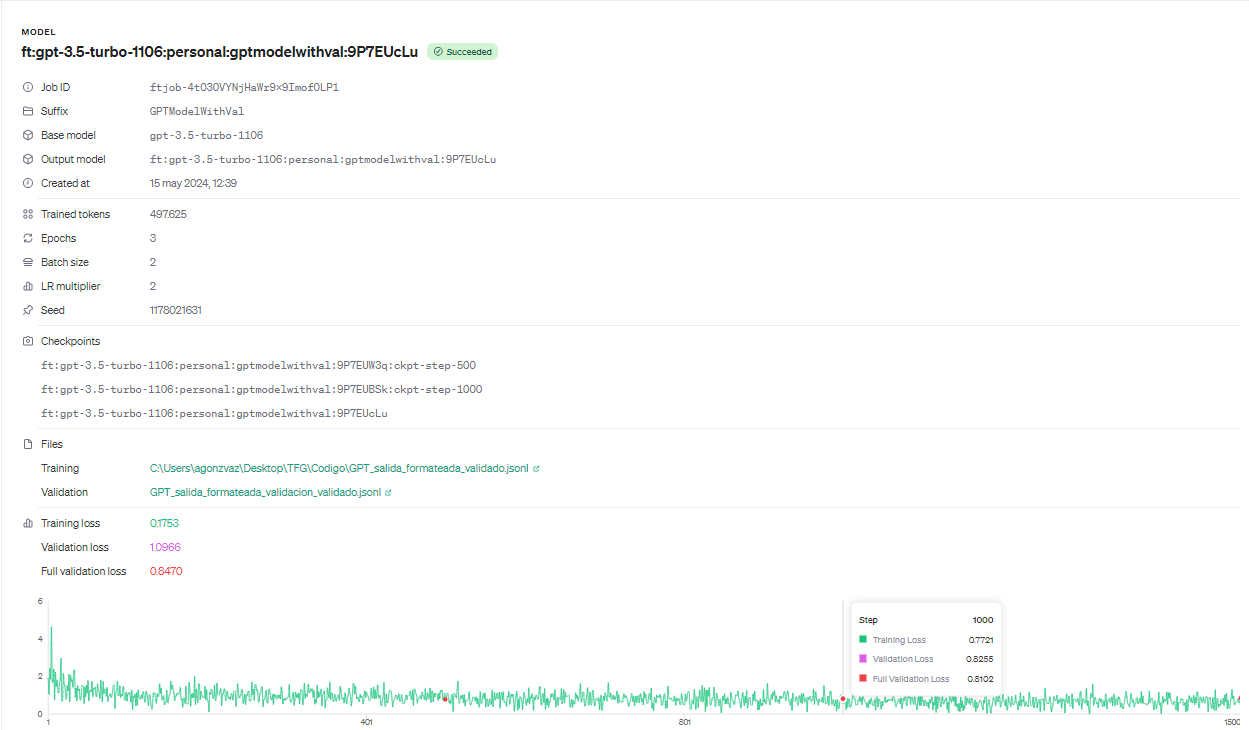
\includegraphics[width=\textwidth,keepaspectratio]{imaxes/5_GPT_EntrenamientoInterfaz.png}
  \caption{Resultado del entrenamiento GPT.}
  \label{fig:5_GPT_EntrenamientoInterfaz}
\end{figure}


\newpage % Fuerza un salto de página
Una vez finalizado el entrenamiento, el modelo puede ser evaluado y ajustado utilizando la interfaz de \acrshort{GPT}. Es posible comparar su rendimiento con otros modelos y experimentar con parámetros como la temperatura, que afecta la creatividad de las respuestas generadas, y el uso de \gls{token}s, que controla la longitud de las respuestas como se muestra en la figura \ref{fig:5_ComparativaModeloGPT}. Estos ajustes permiten optimizar el modelo según las necesidades específicas y mejorar su desempeño en diferentes contextos y aplicaciones.
\bigskip % Deja una línea en blanco

\begin{figure}[htbp!]
  \centering
  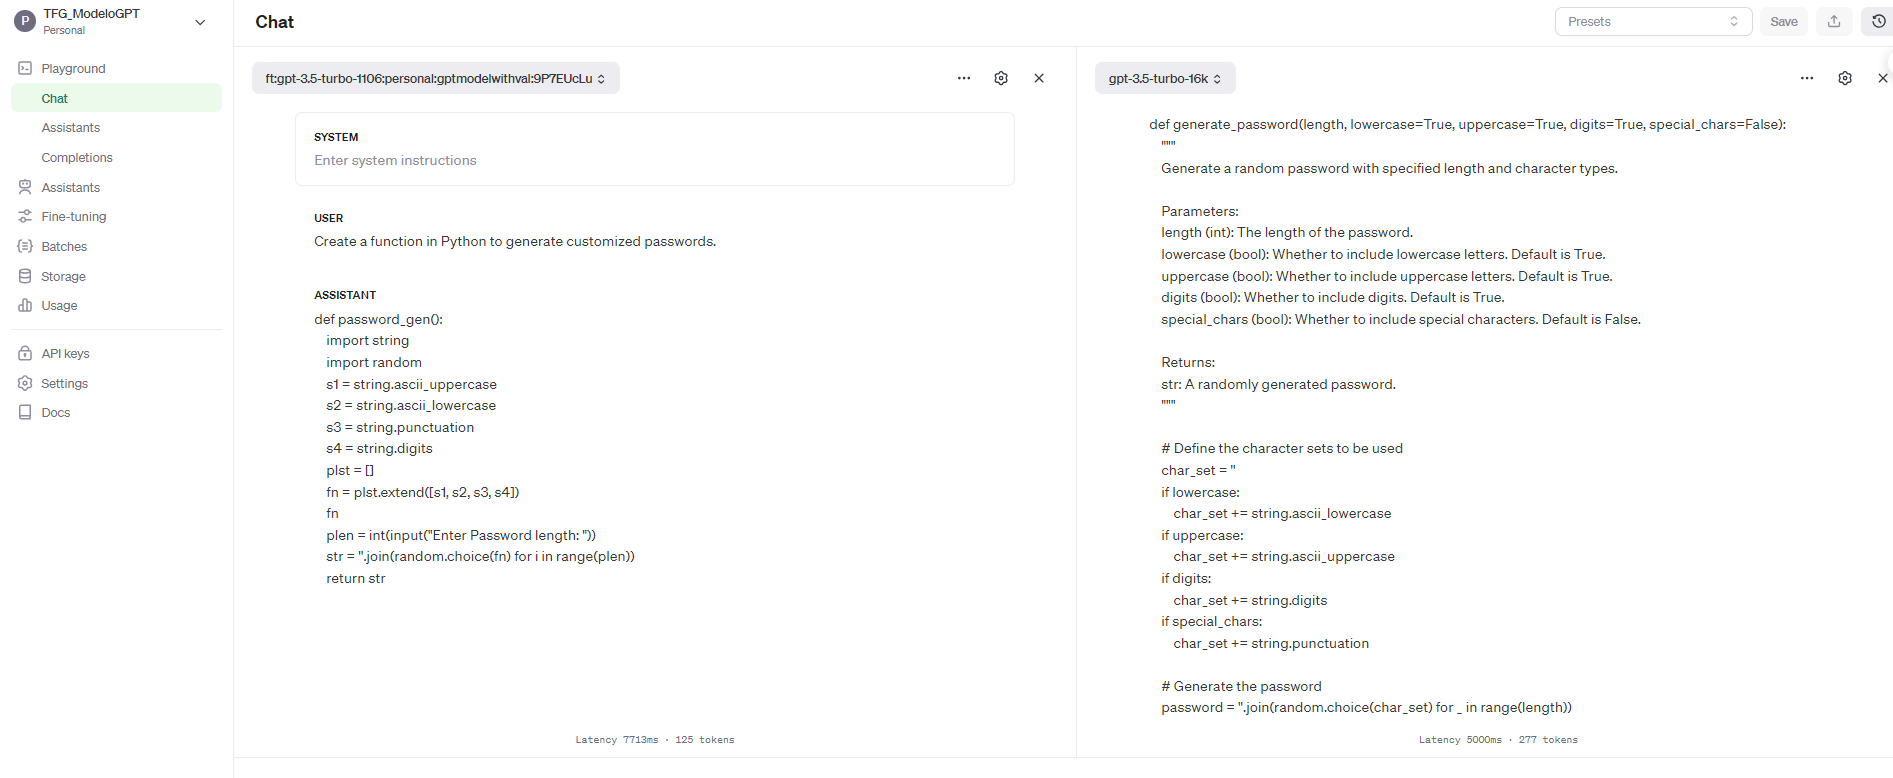
\includegraphics[width=\textwidth,keepaspectratio]{imaxes/5_ComparativaModeloGPT.png}
  \caption{Ejemplo comparativo entre el modelo entrenado y GPT-3.5-Turbo.}
  \label{fig:5_ComparativaModeloGPT}
\end{figure}

En el contexto de nuestra investigación, se identificó que el proceso de tokenización implementado durante el Fine-Tuning del modelo \acrshort{GPT} fue determinante para optimizar la eficiencia y minimizar los costos asociados. El costo total incurrido para el Ajuste Fino de nuestro modelo ascendió a 3.98 dólares \cite{APIOpenApi}, representando una alternativa considerablemente económica en comparación con el uso de modelos más avanzados, como el GPT-3.5 Turbo. La eficiente gestión de tokens facilitó ajustes precisos al modelo, evitando gastos excesivos y preservando la capacidad y robustez del \acrshort{GPT}-3.5 Turbo para su aplicación en nuestro proyecto específico.

\subsection{Modelo LLAMA}

\acrshort{LLaMA} es actualmente uno de los modelos de lenguaje más destacados, desarrollado y liberado por Meta. Similar a \acrshort{GPT}, emplea la arquitectura de Transformers \ref{subsubsec:transformers} para procesar secuencias de texto. El entrenamiento de \acrshort{LLaMA} se divide en dos fases distintas: una fase inicial de preentrenamiento, que se realiza con un extenso conjunto de ejemplos no clasificados para adquirir un conocimiento general del lenguaje, seguida de una fase de Ajuste Fino. Durante el Ajuste Fino, el modelo se especializa en tareas específicas como la clasificación o la comprensión de textos. Esta estructura de entrenamiento permite que \acrshort{LLaMA}  se adapte eficazmente a una amplia gama de aplicaciones lingüísticas, consolidando su posición como un referente en el campo de los modelos de lenguaje a gran escala.

\bigskip % Deja una línea en blanco
En nuestras evaluaciones optamos por \textbf{LLaMA 3}, un modelo recién lanzado que busca superar a sus versiones anteriores en eficiencia y rendimiento. Dos variantes de modelos \acrshort{LLaMA} 3 fueron introducidas basadas en su tamaño: el modelo de 8 mil millones de parámetros (8B) para resultados eficientes y el de 70 mil millones de parámetros (70B) diseñado para tareas complejas. Específicamente, hemos decidido utilizar la versión de \textbf{8B} utilizando el modelo \textbf{unsloth/llama-3-8b-bnb-4bit}, que se encuentra en Hugging Face (\href{https://huggingface.co/unsloth/llama-3-8b-bnb-4bit}{Enlace}).
Se eligió este modelo por su rápido proceso de carga de muestras en el entrenamiento y por las muchas opiniones positivas en el ámbito de modelos de lenguaje a gran escala.

\bigskip % Deja una línea en blanco
Para llevar a cabo este entrenamiento, hemos utilizado un archivo de \textbf{Google Colab} \cite{GoogleColab}  que se encuentra disponible en el enlace proporcionado en relación al modelo elegido anteriormente. Hemos alterado este archivo para adaptarlo a nuestros requerimientos, especialmente por las particularidades de nuestra investigación. Utilizar Google Colab nos brinda la posibilidad de trabajar en un entorno controlado, donde todas las pruebas se llevan a cabo bajo las mismas condiciones en cuanto a memoria, \acrshort{CPU} y versiones de paquetes. Esto asegura un ambiente muy propicio para llevar a cabo comparaciones entre distintos modelos.

\newpage
En primer lugar, comenzamos por la carga de información, para lo cual contamos con un archivo de entrenamiento y otro de validación, ambos en formato \acrshort{JSON}. Estos archivos son fundamentales para los tres entrenamientos que llevaremos a cabo con distintos modelos. Específicamente, \acrshort{LLaMA}  necesita que las muestras sean cargadas de acuerdo a un formato de comando particular, que incluye separadores para distinguir los mensajes y, en cada uno de ellos, el contexto de la salida relacionada.
\bigskip % Deja una línea en blanco

\begin{lstlisting}[language=Python, caption={Conversión JSON a TXT.}, label=listado3]
import json

def transform_conversation(messages):
    reformatted_segments = []

    # We start from 1 because we skip the initial system message
    for i in range(1, len(messages), 2):
        if i + 1 < len(messages) and messages[i]['role'] == 'user' and messages[i+1]['role'] == 'assistant':
            user_text = messages[i]['content']
            assistant_text = messages[i+1]['content']

            # Apply the new template
            reformatted_segments.append(f'<s>[INST] {user_text} [/INST] {assistant_text} </s>')

    return ''.join(reformatted_segments)

# Apply the transformation
transformed_texts = []
for conversation in data['messages']:
    transformed_texts.append(transform_conversation(conversation['messages']))

\end{lstlisting}

\bigskip % Deja una línea en blanco

En la ejecución de esta prueba, empleamos en Google Colab una tarjeta gráfica de aceleración, la GPU A100 de NVIDIA \cite{A100}, conocida por su alta capacidad de cómputo y eficiencia en el procesamiento de operaciones de inteligencia artificial. Este modelo de \acrshort{GPU} facilita el manejo de grandes volúmenes de datos y modelos complejos gracias a su arquitectura optimizada y a su extensa memoria, lo que nos permitió alcanzar resultados eficientes y procesar la gran cantidad de ejemplos de nuestra investigación.

\bigskip % Deja una línea en blanco

Para el ajuste del modelo, utilizamos métodos de Fine-Tuning avanzados, como \gls{QLoRA}, que nos permitió realizar una \textbf{cuantificación} eficiente hasta una precisión de 4 bits sin degradar el rendimiento del modelo. Este método se enfoca en ajustar solamente pequeños adaptadores añadidos al modelo preentrenado, lo cual implica que solo los \gls{gradiente}s de estas capas se actualizan durante el entrenamiento, manteniendo inalterado el resto del modelo congelado de 4 bits. La ventaja de este enfoque es que la \acrshort{VRAM} se utiliza de manera más eficiente y se evita la sobrecarga computacional de entrenar un modelo grande desde cero. El beneficio de esta estrategia radica en la optimización del uso de la \acrshort{VRAM} y en la reducción de la carga computacional al entrenar un modelo extenso desde cero. También, nuestros hallazgos verificaron que la precisión del modelo no se ve impactada por la cuantificación de 4 bits, lo cual confirma la efectividad de \gls{QLoRA} como enfoque de adaptación en contextos de baja precisión numérica.

\bigskip % Deja una línea en blanco

\begin{figure}[htbp!]
  \centering
  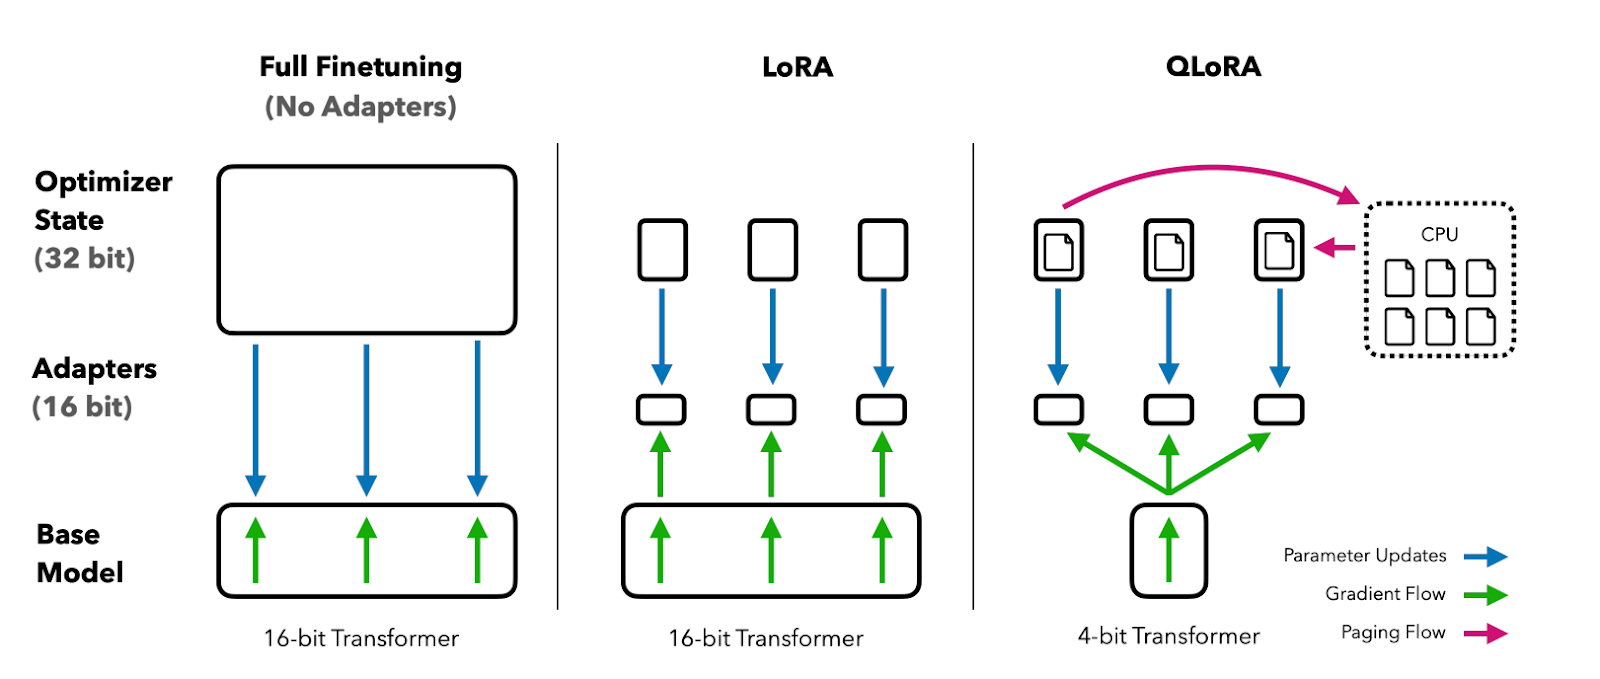
\includegraphics[width=\textwidth,keepaspectratio]{imaxes/5_QLORA.png}
  \caption[Cuantificación de 4 bits mediante QLoRA]{Cuantificación de 4 bits mediante QLoRA. \textit{Fuente: \cite{Mercity2024FineTuning}}}
  \label{fig:5_QLORA.png}
\end{figure}


\bigskip % Deja una línea en blanco

Posteriormente, continuamos con la carga del modelo y la configuración de ciertos parámetros necesarios por QLoRA para asegurar una eficiente configuración. Después, definimos los parámetros de entrenamiento. Es crucial mencionar que hemos realizado entrenamientos similares para no afectar los datos resultantes, ya que planeamos comparar otros modelos en el futuro. Para asegurar la coherencia, hemos utilizado los valores de los parámetros del modelo \acrshort{GPT} mencionados en la sección previa (ver Subsección \ref{subsec:modelogpt}). También analizaremos la utilización del gradiente, el cual será utilizado para reducir una función de pérdida que evalúa la discrepancia entre las predicciones del modelo y los valores reales, modificando los parámetros del modelo, como los pesos en una red neuronal.

\bigskip % Deja una línea en blanco

Como consecuencia, se obtiene la tabla mencionada en la referencia \ref{fig:5_LLAMA_TablaSteps.png}, la cual exhibe los resultados alcanzados en las distintas etapas del procedimiento. Este cuadro es esencial para medir el desempeño del modelo en cada etapa de entrenamiento y facilita la comparación del efecto de los cambios realizados en los parámetros.


\clearpage  % Esto fuerza a LaTeX a colocar todas las figuras pendientes y comenzar en una nueva página

\begin{figure}[htbp!]
  \centering
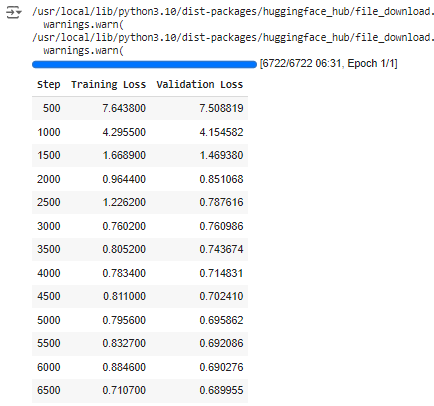
\includegraphics[width=0.8\textwidth,keepaspectratio]{imaxes/5_LLAMA_TablaSteps.png}
  \caption{Tabla con resultados del entrenamiento y validación de LLAMA 3.}
  \label{fig:5_LLAMA_TablaSteps.png}
\end{figure}

\bigskip % Deja una línea en blanco

Al igual que con \acrshort{GPT}, hemos decidido mostrar una representación visual de los resultados, incluyendo las etapas de entrenamiento y validación. Este gráfico ayuda a entender cómo se comporta el modelo a lo largo del tiempo y permite evaluar de forma más intuitiva su rendimiento en distintas etapas.

\bigskip % Deja una línea en blanco

\begin{figure}[htbp!]
  \centering
  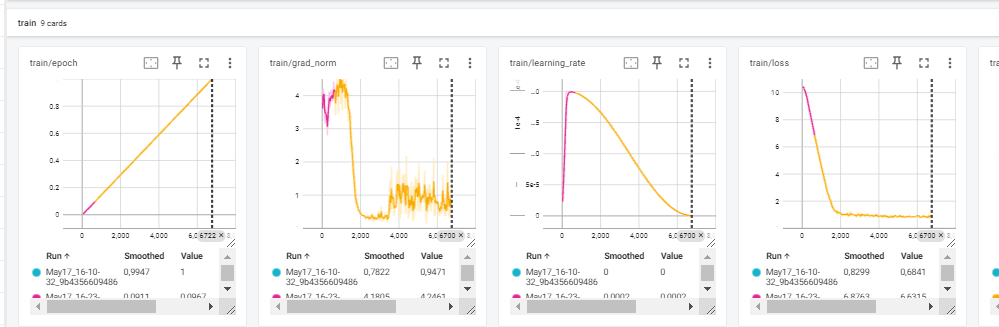
\includegraphics[width=\textwidth,keepaspectratio]{imaxes/5_LLAMA_Graficos_Train.png}
  \caption{Gráfica con los resultados del entrenamiento en LLAMA 3.}
  \label{fig:5_LLAMA_Graficos_Train.png}
\end{figure}

\bigskip % Deja una línea en blanco

Podemos observar en las secciones anteriores las diferentes gráficas \ref{fig:5_LLAMA_Graficos_Train.png} que representan diversos aspectos del entrenamiento:

\begin{itemize}
    \item \textbf{Epoch (train/epoch):} El gráfico muestra un aumento lineal en el número de epochs, lo que es esperado ya que representa el progreso del entrenamiento.

    \item \textbf{Norma del Gradiente (train/grad\_norm):} El valor de la norma del gradiente es volátil al principio pero luego se estabiliza. Altos valores iniciales y fluctuaciones pueden indicar ajustes grandes en los pesos del modelo, que luego se suavizan.

    \item \textbf{Tasa de Aprendizaje (train/learning\_rate):} La tasa de aprendizaje disminuye dramáticamente después de cierto punto, lo cual es típico de los esquemas de reducción de la tasa de aprendizaje para ayudar al modelo a converger mejor hacia el final del entrenamiento.

    \item \textbf{Loss de Entrenamiento (train/loss):} La pérdida de entrenamiento disminuye de manera constante, lo que indica un buen aprendizaje durante las \textit{epochs}. La tendencia descendente es un buen signo de que el modelo está aprendiendo adecuadamente.
\end{itemize}

\bigskip % Deja una línea en blanco

De igual forma, se pueden observar \ref{fig:5_LLAMA_Grafico_Val.png}{} los aspecto del proceso de evaluación realizado:

\begin{figure}[htbp!]
  \centering
  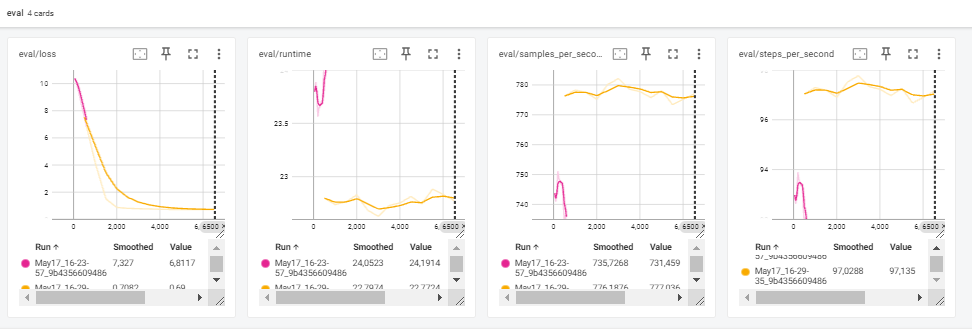
\includegraphics[width=\textwidth,keepaspectratio]{imaxes/5_LLAMA_Grafico_Val.png}
  \caption{Gráfica con los resultados de la validación de LLAMA 3.}
  \label{fig:5_LLAMA_Grafico_Val.png}
\end{figure}

\bigskip % Deja una línea en blanco

\begin{itemize}
    \item \textbf{Loss de Evaluación (eval/loss):} La pérdida disminuye significativamente y de forma estable a lo largo de las iteraciones, lo que indica que el modelo está aprendiendo y mejorando su rendimiento en los datos de validación.

    \item \textbf{Tiempo de Ejecución por Evaluación (eval/runtime):} Hay fluctuaciones en el tiempo de ejecución, pero parece estabilizarse hacia el final. No hay indicios claros de problemas como fugas de memoria que podrían aumentar el tiempo de ejecución con más iteraciones.

    \item \textbf{Muestras por Segundo (eval/samples\_per\_second):} Este valor se mantiene bastante estable, aunque hay un pico visible en la gráfica. Esto podría indicar un momento de optimización o ajuste en el proceso de evaluación.

    \item \textbf{Pasos por Segundo (eval/steps\_per\_second):} Similar a las muestras por segundo, es bastante estable, lo cual es positivo porque muestra consistencia en la velocidad de procesamiento del modelo durante la evaluación.
\end{itemize}

\bigskip % Deja una línea en blanco

El entrenamiento de \acrshort{LLaMA} 3 ha sido exitoso y eficaz, como se evidencia por la constante y notable disminución de la pérdida observada en las etapas de entrenamiento y evaluación. Esto indica que el modelo ha aprendido de manera efectiva, ya que la pérdida ha disminuido. Además, \acrshort{LLaMA} 3 ha demostrado ser estable en cuanto a su tiempo de ejecución y procesamiento. Hacer cambios en la tasa de aprendizaje y regular la norma del gradiente pueden mejorar la configuración de los parámetros para optimizar de manera efectiva. Estos hallazgos destacan que \acrshort{LLaMA} 3 es un modelo sólido y capaz, listo para ser utilizado con éxito en labores de procesamiento del lenguaje.
\bigskip % Deja una línea en blanco


Por último, debido al entorno de código abierto de este proceso de capacitación, se ha optado por compartir el modelo entrenado y los conjuntos de datos en la plataforma de Hugging Face (\href{https://huggingface.co/eibeel/llama3_python_TFG}{Enlace}) con el objetivo de respaldar y promover el desarrollo de modelos de código abierto. Esta es una muy buena alternativa para hacer pruebas con los modelos empleando herramientas como LM Studio \cite{LMStudio}, donde es posible descargar los modelos elegidos y hacer peticiones para comparar sus resultados.
\bigskip % Deja una línea en blanco

\subsection{Modelo Mixtral}

En esta sección, analizaremos nuestro proyecto utilizando \textbf{Mixtral}, un modelo de lenguaje creado por la empresa emergente francesa Mistral AI. Este proyecto fue establecido en abril de 2023 por antiguos trabajadores de Meta y Google. Indudablemente, Mixtral es uno de los modelos más prometedores en la actualidad, equiparable a \acrshort{GPT} y \acrshort{LLaMA}, y puede manejar cantidades de datos considerablemente más grandes. Mixtral se distingue por ser de código abierto.

\bigskip % Deja una línea en blanco

La estructura de entrenamiento de Mixtral es fundamental para su éxito, ya que garantiza resultados rápidos y eficientes. Esto se logra gracias al sistema \acrfull{MoE}.

\bigskip % Deja una línea en blanco

Un sistema \acrshort{MoE} \cite{MistureExperts} es una técnica utilizada en el área de los modelos de lenguaje que fragmenta un modelo extenso en múltiples submodelos más reducidos, cada uno enfocado en un conjunto particular de funciones. Esta especialización mejora la eficiencia y efectividad del sistema en la gestión de diversas tareas.

\bigskip % Deja una línea en blanco

La entrada se transforma en un vector con sus propias características \ref{fig:5_MIXTRAL_MoE}, que posteriormente se introduce en la red de enrutamiento. En este momento, es necesario determinar a cuáles modelos enviar la entrada, basándose en cuáles de ellos producirán la salida óptima. Para seleccionar, se asigna una puntuación a cada submodelo de \acrshort{MoE}, indicando su habilidad para abordar la tarea según su especialización. Una vez se obtienen estas calificaciones, el router selecciona los submodelos más competentes, aquellos con la mejor calificación, para llevar a cabo la tarea, combinando al final sus resultados para producir el resultado final, conocido como \textit{ensemble} en el campo del Machine Learning. En el nuevo modelo de Mistral, se eligen los dos modelos más competentes.

\bigskip % Deja una línea en blanco


\begin{figure}[ht!]
  \centering
  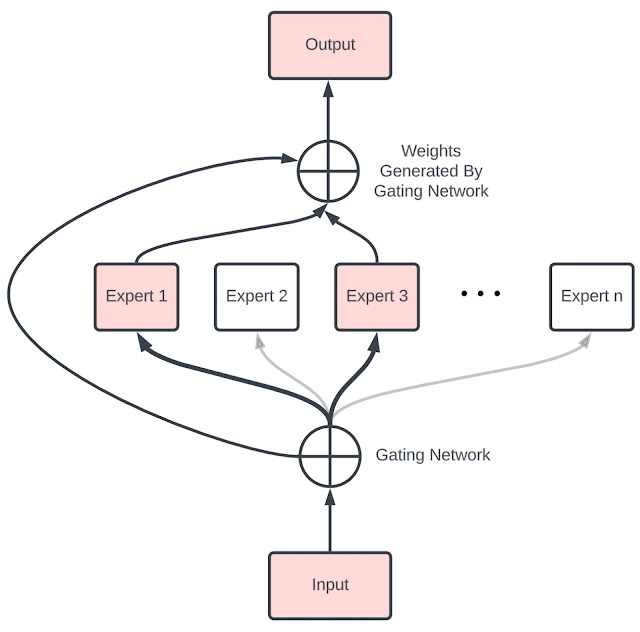
\includegraphics[width=0.5\textwidth, keepaspectratio]{imaxes/5_MIXTRAL_MoE.jpg}
  \caption[Arquitectura Mixture of Experts]{Arquitectura Mixture of Experts. \textit{Fuente: \cite{Elmo2024Mixtral}}}
  \label{fig:5_MIXTRAL_MoE}
\end{figure}



\bigskip % Deja una línea en blanco

En nuestra selección, elegimos \textbf{Mixtral-8x7B}, que salió al mercado recientemente. Es uno de los modelos de código abierto más poderosos en la actualidad, incluso comparable con los modelos destacados de OpenAI y Meta. En este momento, existen diversas variantes de Mixtral, como la modalidad con un único modelo de 7 mil millones de parámetros (más eficaz) y las modalidades con varios modelos, como las de 8x7 mil millones de parámetros y 8x22 mil millones de parámetros. Indudablemente, el ámbito open source está empezando a competir con compañías de gran tamaño. En nuestra situación, por la falta de recursos, hemos elegido trabajar con la versión de 8x7B, utilizando el modelo \textbf{mistralai/Mistral-7B-Instruct-v0.1}.

\bigskip % Deja una línea en blanco

Durante la ejecución del entrenamiento, hemos decidido utilizar Google Colab ya que permite sacar mayor provecho de los recursos disponibles en comparación con los de nuestra propia computadora portátil. Para lograrlo, hemos tomado como referencia los pasos de la sección \ref{subsec:modelogpt}, puesto que el propósito del proyecto es poder obtener conclusiones comparativas de los tres modelos en situaciones parecidas.

\bigskip % Deja una línea en blanco

Iniciamos primero con la carga de información. En esta etapa, no se han requerido efectuar cambios en los archivos de datos, ya que hemos utilizado los archivos en formato txt previamente utilizados. Mixtral no especifica un requisito en el formato del \textit{prompt}, pero sí recomienda seguir los patrones que actualmente se emplean, diferenciando el texto de usuario y el de asistente.

\bigskip % Deja una línea en blanco

El uso de \textit{padding} es frecuente en el procesamiento de \acrshort{NLP} para garantizar que todas las secuencias de entrada tengan la misma longitud. Esto es fundamental en el procesamiento por lotes, ya que es imprescindible que las secuencias tengan longitudes uniformes para que los modelos de aprendizaje automático puedan procesarlas eficazmente.

\bigskip % Deja una línea en blanco

En el caso de Mixtral, lo hemos aplicado de la siguiente forma:

\bigskip % Deja una línea en blanco

\begin{lstlisting}[language=Python, caption={Parámetro de padding.}, label=listado4]
try:
    # Attempt to load the tokenizer
    tokenizer = AutoTokenizer.from_pretrained(model_id, force_download=True)
    tokenizer.pad_token = tokenizer.unk_token
    tokenizer.pad_token_id = tokenizer.unk_token_id
    tokenizer.padding_side = 'right'
    print("Tokenizer loaded successfully.")

    # Attempt to load the model
    model = AutoModelForCausalLM.from_pretrained(model_id, force_download=True)
    print("Model loaded successfully.")
except Exception as e:
    print(f"Error loading the tokenizer or model: {e}")
\end{lstlisting}

\bigskip % Deja una línea en blanco

Es relevante destacar que utilizamos los mismos recursos que en versiones anteriores, como la tarjeta de aceleración gráfica, la \textbf{GPU A100}. Además, emplearemos la misma configuración y métodos de capacitación. Utilizando el Fine-Tuning, readoptaremos la técnica eficaz de \acrshort{QLoRA} para ajustar el modelo a una precisión de 4 bits y aumentar la eficiencia aún más.

\bigskip % Deja una línea en blanco

Después de cargar los datos y el modelo, ahora vamos a ajustar los parámetros de entrenamiento para asegurarnos de tener las mismas condiciones que en modelos previos y poder hacer comparaciones válidas.
A continuación, se presenta esta disposición para comprender minuciosamente los campos y valores asociados.

\bigskip % Deja una línea en blanco

\begin{lstlisting}[language=Python, caption={Argumentos del entrenamiento.}, label=listado5]
training_arguments = TrainingArguments(
        output_dir="./results_mixtral_sft/",
        evaluation_strategy="steps",
        do_eval=True,
        optim="paged_adamw_8bit",
        num_train_epochs=1,
        per_device_train_batch_size=4,
        gradient_accumulation_steps=2,
        per_device_eval_batch_size=4,
        log_level="debug",
        save_steps=1000,
        logging_steps=logging_steps,
        learning_rate=2e-4,
        eval_steps=500,
        max_steps=-1,
        lr_scheduler_type="linear",
        report_to="tensorboard"  
)
\end{lstlisting}

\bigskip % Deja una línea en blanco

Algunos de los argumentos anteriores con mayor relevancia son:

\begin{itemize}
    \item \textbf{Evaluation\_strategy}: Evalúa el modelo cada cierto número de pasos.
    \item \textbf{Do\_eval}: Indica si se debe realizar la evaluación durante el entrenamiento.
    \item \textbf{Num\_train\_epochs}: Número de épocas de entrenamiento.
    \item \textbf{Per\_device\_train\_batch\_size}: Tamaño del \textit{batch} de entrenamiento por dispositivo (GPU/CPU).
    \item \textbf{Gradient\_accumulation\_steps}: Número de pasos de acumulación de gradientes antes de realizar una actualización de parámetros.
    \item \textbf{Per\_device\_eval\_batch\_size}: Tamaño del \textit{batch} de evaluación por dispositivo.
    \item \textbf{Max\_steps}: Número máximo de pasos de entrenamiento. \textbf{-1} indica que no hay límite máximo de pasos, se entrenará por el número de épocas especificadas.
    \item \textbf{Lr\_scheduler\_type}: Tipo de programador de tasa de aprendizaje. "\textit{linear}" reduce la tasa de aprendizaje linealmente a lo largo del entrenamiento.
\end{itemize}


\bigskip % Deja una línea en blanco

Después de completar la capacitación, se accede a los datos de la tabla mencionada en \ref{fig:5_LLAMA_TablaSteps.png}, lo que permite visualizar los resultados en cada fase. En esa tabla se puede ver cómo funciona el modelo durante las etapas de entrenamiento y validación.

\bigskip % Deja una línea en blanco

\begin{figure}[htbp!]
  \centering
  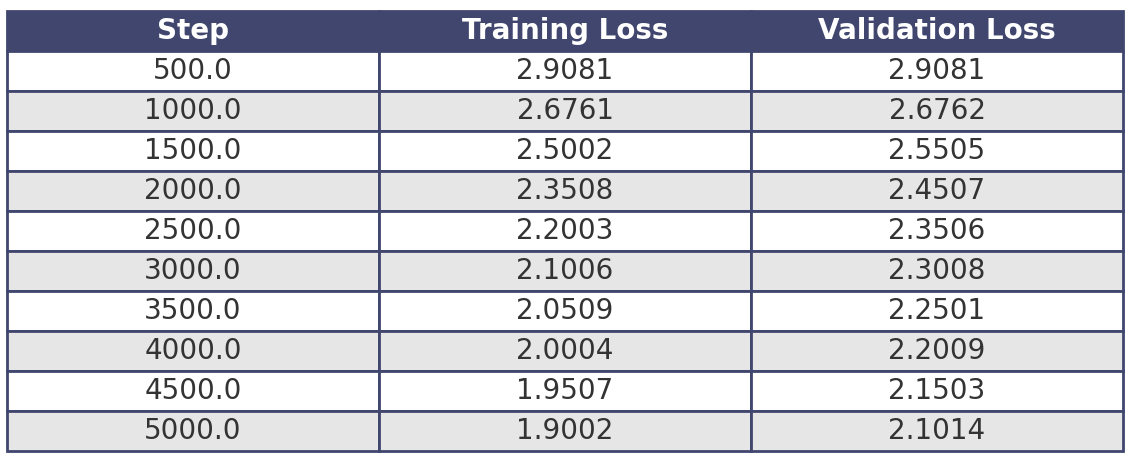
\includegraphics[width=\textwidth,keepaspectratio]{imaxes/5_MIXTRAL_TablaTeps.png}
  \caption{Tabla con resultados del entrenamiento y validación en MIXTRAL.}
  \label{fig5_MIXTRAL_TablaTeps}
\end{figure}

\bigskip % Deja una línea en blanco

Al igual que en las situaciones previas, hemos decidido mostrar de manera visual los resultados de las fases de entrenamiento y validación. Esto nos permitirá comprender la forma en que nuestro modelo se comporta frente a los datos dados.

\bigskip % Deja una línea en blanco

\begin{figure}[htbp!]
  \centering
  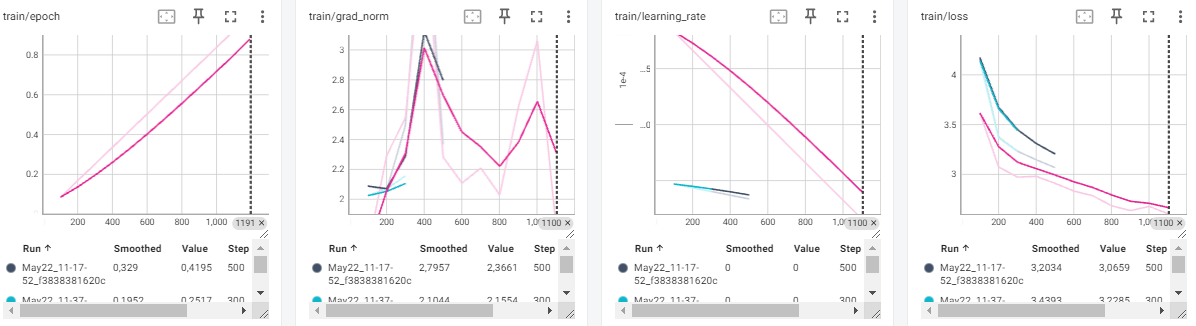
\includegraphics[width=\textwidth,keepaspectratio]{imaxes/5_MIXTRAL_Grafico_Train.png}
  \caption{Gráfica con los resultados del entrenamiento en MIXTRAL.}
  \label{fig:5_MIXTRAL_Grafico_Train}
\end{figure}

\bigskip % Deja una línea en blanco

\begin{itemize}
    \item \textbf{Epoch (train/epoch):} La evolución del entrenamiento según las épocas sigue una tendencia lineal, lo que sugiere que el modelo está adquiriendo conocimiento de forma constante a lo largo del tiempo, cumpliendo con las expectativas durante el proceso de entrenamiento.
    \item \textbf{Norma del Gradiente (train/grad\_norm):} La representación visual del gradiente de la norma presenta variaciones, con un punto más alto al principio y disminuciones después. Esta situación es típica, ya que el modelo modifica los gradientes mientras se entrena para reducir la pérdida. Los picos pueden señalar instantes en los que el modelo hizo cambios importantes en los pesos.
    \item \textbf{Tasa de Aprendizaje (train/learning\_rate):} La disminución de la tasa de aprendizaje se representa en la gráfica de forma exponencial. Una técnica habitual para garantizar que el modelo realice ajustes más precisos a medida que se acerca al mínimo de pérdida es la disminución de la tasa de aprendizaje.
    \item \textbf{Loss de Entrenamiento (train/loss):} El gráfico de la disminución de la pérdida durante el entrenamiento revela una evidente disminución, lo que sugiere una mejora en el rendimiento del modelo a lo largo del tiempo. La disminución de la pérdida se reduce rápidamente al principio y luego se estabiliza, un patrón común en el aprendizaje de modelos en las primeras etapas.
\end{itemize}

\bigskip % Deja una línea en blanco

De igual forma podemos observar \ref{fig:5_MIXTRAL_Grafico_Val} el proceso de evaluación realizado:

\bigskip % Deja una línea en blanco

\begin{figure}[htbp!]
  \centering
  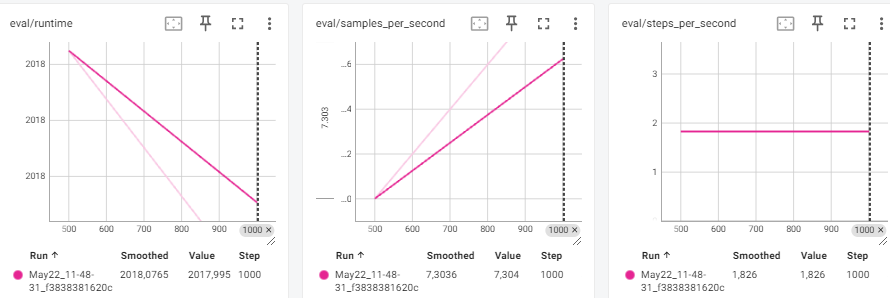
\includegraphics[width=\textwidth,keepaspectratio]{imaxes/5_MIXTRAL_Grafico_Val.png}
  \caption{Gráfica con los resultados de la validación en MIXTRAL.}
  \label{fig:5_MIXTRAL_Grafico_Val}
\end{figure}

\bigskip % Deja una línea en blanco

\begin{itemize}
    \item \textbf{Tiempo de Ejecución por Evaluación (eval/runtime):} Esto sugiere que la eficacia del proceso de validación está mejorando con el tiempo, probablemente gracias a mejoras internas y estabilidad en las fases finales del entrenamiento.
    \item \textbf{Muestras por Segundo (eval/samples\_per\_second):} Esto indica que el modelo está progresando en cuanto a eficiencia de procesamiento, siendo capaz de procesar una mayor cantidad de datos en menos tiempo a medida que avanza el entrenamiento.
    \item \textbf{Pasos por Segundo (eval/steps\_per\_second):} Esto indica una consistencia positiva en el desempeño del modelo durante la validación, lo cual es un buen signo de estabilidad.
\end{itemize}

\bigskip % Deja una línea en blanco

Según las gráficas (\ref{fig:5_MIXTRAL_Grafico_Train} y \ref{fig:5_MIXTRAL_Grafico_Val}) y la tabla (\ref{fig:5_LLAMA_TablaSteps.png}), se sugiere que el modelo \textbf{MIXTRAL} ha sido entrenado de manera eficiente, logrando reducir el tiempo de ejecución y aumentar la velocidad de procesamiento de las muestras. Esto señala un proceso de entrenamiento y validación optimizado. La disminución de la pérdida en entrenamiento y validación es constante, lo que sugiere que el modelo está aprendiendo de manera efectiva y generalizando correctamente a los datos de validación. Asimismo, la regla del gradiente y la velocidad de aprendizaje presentan comportamientos predecibles que favorecen la convergencia del modelo, y la consistencia en los pasos por segundo durante la validación respalda esta afirmación. En resumen, parece que el entrenamiento del modelo MIXTRAL fue efectivo, demostrando un buen desempeño y estabilidad durante cada etapa, indicando una optimización eficiente en el procesamiento de datos.

\bigskip % Deja una línea en blanco.

Por último, llevar a cabo pruebas en este proyecto de código abierto sugiere que proyectos como \acrshort{GPT} y \acrshort{LLaMA} no están muy lejos en comparación con MIXTRAL. De la misma manera que hicimos en ejemplos anteriores, pondremos tanto el modelo entrenado como los datos empleados en la plataforma de Hugging Face (\href{https://huggingface.co/eibeel/mixtral_tfg}{Enlace}) para continuar contribuyendo al desarrollo de software de código abierto.


\subsection{Evaluación de modelos y comparativa de resultados}
\label{subsec:evaluaciónmodelos}

En esta sección examinaremos los resultados de los modelos con métricas y métodos diferentes para determinar cuál es el más adecuado para nuestras necesidades. La valoración y el estudio de modelos, como \acrshort{GPT}, \acrshort{LLaMA} y MIXTRAL, son fundamentales en inteligencia artificial para garantizar su eficacia y exactitud en funciones como la redacción de texto, traducción automática, síntesis de textos y resolución de preguntas.

\bigskip % Deja una línea en blanco.

Una investigación reciente \cite{hassid2024larger} indica que modelos con menos parámetros (7 mil millones y 13 mil millones) pueden ser más efectivos que modelos con más parámetros (34 mil millones y 70 mil millones) en tareas de generación de código con el mismo costo computacional. En este \acrshort{TFG}, utilizaremos medidas como \acrshort{BLEU} y ROUGE para valorar los modelos, investigando si la repetición de la ejecución de modelos pequeños podría ser más efectiva que el empleo de modelos grandes.

\bigskip % Deja una línea en blanco

Primero, optamos por llevar a cabo varios experimentos con las predicciones de los modelos ensayados. Para ello, damos a nuestros modelos un \textit{prompt} que indica lo requerido y la respuesta deseada. De acuerdo a las especificaciones de cada modelo, podremos notar las disparidades entre ellos y tener una clara noción de cuál es el más adecuado para nuestro problema.

\bigskip % Deja una línea en blanco

\begin{lstlisting}[language=Python, caption={Prompt y salida de referencia.}, label=listado6]
def main():
    # Prompt para generar el código Python
    prompt = "Write a Python function that sums all prime numbers from 1 to 1000."

    # Generar predicción
    candidate = generate_predictions(model, prompt)
    print(f"Generated code:\n{candidate}")

    # Respuesta de referencia esperada (en inglés)
    reference = """
def sum_primes():
    def is_prime(n):
        if n <= 1:
            return False
        for i in range(2, int(n**0.5) + 1):
            if n % i == 0:
                return False
        return True

    total = sum(n for n in range(2, 1001) if is_prime(n))
    return total

print(sum_primes())
""".strip()

\end{lstlisting}

\bigskip % Deja una línea en blanco

A continuación, se presentará la salida producida por cada modelo con el fin de visualizar las disparidades entre ellos. Claramente, cada modelo exhibe sus propias características al abordar la cuestión que hemos planteado a través del \textit{prompt}.
\begin{itemize}
    \item \textbf{\acrshort{GPT}}: 

    \begin{lstlisting}[language=Python, caption={Salida generada por GPT.}, label=listado7]
    def isPrime(n):
        if(n<2): return False
        if(n==2): return True
        if(n%2==0): return False
        for i in range(3,int(n**0.5)+1,2):
            if(n%i==0):
                return False            
        return True

    def sum_primes(n):
     return sum([i for i in range(n + 1) if isPrime(i)])

    sum_primes(1000)
    \end{lstlisting}

    
    \item \textbf{\acrshort{LLaMA}}:

    \begin{lstlisting}[language=Python, caption={Salida generada por LLaMA.}, label=listado8]
    def sum_primes(n):
        def is_prime(num):
            if num < 2:
            return False
            for i in range(2, int(num**0.5) + 1):
                if num % i == 0:
            return False
            return True

        return sum(i for i in range(2, n+1) if is_prime(i))

    print(sum_primes(1000))
    \end{lstlisting}
    
\item \textbf{MIXTRAL}:

    \begin{lstlisting}[language=Python, caption={Salida generada por MIXTRAL.}, label=listado9]
    def sum_primes():
        def is_prime(n):
            if n <= 1:
                return False
            for i in range(2, int(n**0.5) + 1):
                if n % i == 0:
                    return False
return True

total = sum(n for n in range(2, 1001) if is_prime(n))
        return total

    print(sum_primes())
    \end{lstlisting}
\end{itemize}

Para asegurar una revisión detallada del modelo, establecimos medidas como exactitud, recordatorio, puntuación F1 y \acrshort{BLEU}. Estas medidas nos dan un valor numérico del desempeño del modelo en actividades concretas, lo que nos habilita para cotejar distintos modelos o modificaciones de hiperparámetros.

\begin{itemize}

\item\textbf{Precisión (Precision):} Este indicador evalúa la fracción de predicciones positivas acertadas de todas las predicciones positivas hechas por el modelo. En otras palabras, la precisión mide la cantidad de elementos clasificados como positivos que son verdaderamente positivos. Se estima con la fórmula:
    
\[
\text{Precisión} = \frac{\text{Verdaderos Positivos}}{\text{Verdaderos Positivos} + \text{Falsos Positivos}}
\]

    En un caso de clasificación binaria, la precisión indica cuántos de los casos identificados como positivos por el modelo son realmente positivos.

    \bigskip % Deja una línea en blanco

\item \textbf{Recuperación (Recall):} Esta métrica evalúa cuántos ejemplos positivos son identificados correctamente por el modelo en comparación con el total de ejemplos positivos presentes en el conjunto de datos. En otras términos, la recuperación indica la cantidad de elementos positivos reales que fueron correctamente reconocidos por el modelo. La fórmula se utiliza para el cálculo.
    
\[
\text{Recuperación} = \frac{\text{Verdaderos Positivos}}{\text{Verdaderos Positivos} + \text{Falsos Negativos}}
\]
    
En el caso de un problema de detección de correo no deseado, la recuperación nos proporcionará información sobre la cantidad de correos electrónicos identificados como correo no deseado por el modelo en comparación con todos los correos no deseados en el conjunto de datos.

\bigskip % Deja una línea en blanco
    
\item \textbf{Puntuación F1 (F1 Score):} Esta métrica combina la exactitud y la recuperación en un solo valor que brinda una evaluación más equilibrada de la eficacia del modelo. Resulta especialmente beneficioso cuando existe una falta de equilibrio en la distribución de clases en los datos. La F1 score se calcula como el promedio armónico de precisión y recall, y se define mediante esta fórmula:
\[
\text{Puntuación F1} = 2 \times \frac{\text{Precisión} \times \text{Recuperación}}{\text{Precisión} + \text{Recuperación}}
\]

La puntuación F1 alcanza su mejor valor en 1 (indicando una precisión perfecta y una recuperación perfecta) y su peor valor en 0 (indicando un rendimiento pobre en ambas métricas). Esta métrica es útil cuando nos interesa encontrar un equilibrio entre la precisión y la recuperación en la evaluación del modelo.

\bigskip % Deja una línea en blanco

\item \textbf{\acrfull{BLEU}:} Es una métrica utilizada para evaluar la calidad de texto generado automáticamente, como traducciones automáticas, comparándolo con una o más traducciones de referencia realizadas por humanos. BLEU mide la precisión de n-gramas, es decir, secuencias de palabras de longitud n, para ver cuántos de los n-gramas en el texto generado aparecen también en el texto de referencia. Para ello, se emplea la siguiente fórmula:


\begin{equation}
BLEU = BP \cdot \exp \left( \sum_{n=1}^{N} w_n \log p_n \right)
\end{equation}

\begin{itemize}
    \item \textbf{BP} es la penalización por longitud (Brevity Penalty).
    \item \( N \) es el máximo tamaño de los n-gramas (usualmente hasta 4).
    \item \( w_n \) es el peso asignado a la precisión de n-gramas de tamaño \( n \) (comúnmente iguales para todos los n-gramas).
    \item \( p_n \) es la precisión de los n-gramas de tamaño \( n \).
\end{itemize}

Por lo tanto, \acrshort{BLEU} es un número entre cero y uno que mide la similitud del texto traducido de manera automática con un conjunto de traducciones de referencia de alta calidad.

\end{itemize}

En nuestro estudio, una vez hemos realizado los entrenamientos con los diferentes modelos hemos obtenido una serie de resultados en función de como había sido el entrenamiento (secciones anteriores). Llegados a este punto, hemos decidido realizar un análisis más profundo respecto a la evaluación de los modelos, por lo que nos hemos centrado en las métricas comentadas anteriormente. Para la realización de este proceso hemos creado un único conjunto de datos que le hemos pasado a los diferentes modelos para obtener mayor información respecto al entrenamiento.

\bigskip % Deja una línea en blanco

En la investigación, después de completar los entrenamientos con los distintos modelos, hemos conseguido una variedad de resultados basados en la forma en que se llevó a cabo el entrenamiento. En este punto, hemos optado por llevar a cabo un examen más detallado sobre la evaluación de los modelos, enfocándonos en las métricas previamente mencionadas. Para llevar a cabo este procedimiento, hemos desarrollado un único \textit{script} que hemos proporcionado a los diversos modelos con el fin de obtener más datos sobre el proceso de entrenamiento.

\bigskip % Deja una línea en blanco

El \textit{script} consta de lo siguiente, a mayores de las librerías propias de cada modelo como pueden ser la de OpenAI o Huggin Face:

\bigskip % Deja una línea en blanco

\begin{lstlisting}[language=Python, caption={Script de evaluación del modelo.}, label=listado10]
import nltk
from nltk.translate.bleu_score import sentence_bleu, SmoothingFunction
from sklearn.metrics import precision_score, recall_score, f1_score

def generate_predictions(model, prompt):
    response = openai.Completion.create(
        model=model,
        prompt=prompt,
        max_tokens=150
    )
    prediction = response.choices[0].text.strip()
    return prediction

def calculate_bleu(references, candidates):
    smooth = SmoothingFunction().method1
    bleu_scores = [sentence_bleu([ref.split()], cand.split(), smoothing_function=smooth) for ref, cand in
                   zip(references, candidates)]
    average_bleu = sum(bleu_scores) / len(bleu_scores)
    return bleu_scores, average_bleu

def calculate_classification_metrics(y_true, y_pred):
    precision = precision_score(y_true, y_pred, average='weighted')
    recall = recall_score(y_true, y_pred, average='weighted')
    f1 = f1_score(y_true, y_pred, average='weighted')
    return precision, recall, f1

\end{lstlisting}

\bigskip % Deja una línea en blanco

A partir del \textit{script} anterior, se presenta la tabla \ref{tab:ComparacionModelos} para facilitar la visualización de los resultados y realizar análisis de los diferentes modelos evaluados.

\bigskip % Deja una línea en blanco

\begin{table}[ht!]
  \centering
  \scalebox{0.90}{ % Cambia el valor 0.90 para ajustar el tamaño
    \rowcolors{2}{white}{gray!25}
    \begin{tabular}{c|c|c|c|c}
      \rowcolor{pink!25}
      \textbf{Modelos} & \textbf{Precision} & \textbf{Recall} & \textbf{F1 Score} & \textbf{\acrshort{BLEU}} \\\hline
      Modelo \acrshort{GPT} & 0.600 & 0.600 & 0.600 & 0.700 \\
      Modelo \acrshort{LLaMA} & 0.486 & 0.486 & 0.486 & 0.568 \\
      Modelo MIXTRAL & 0.857 & 0.857 & 0.857 & 0.943 \\
    \end{tabular}
  }
  \caption{Tabla de comparación de modelos.}
  \label{tab:ComparacionModelos}
\end{table}

\bigskip % Deja una línea en blanco

Al examinar la tabla mencionada \ref{tab:ComparacionModelos}, la comparación entre los modelos proporciona datos significativos sobre su eficacia durante la fase de entrenamiento. Así que analizaremos cada métrica y hablaremos sobre las conclusiones que podemos extraer de ellas.

\bigskip % Deja una línea en blanco

En cuanto a la \textbf{\textit{precision}}, que mide la correcta clasificación de las instancias, se puede notar que el modelo MIXTRAL logra un alto porcentaje de aciertos. Además, \acrshort{GPT} muestra un nivel de rendimiento moderado, mientras que \acrshort{LLaMA} tiene un desempeño significativamente inferior en comparación con los otros modelos.

\bigskip % Deja una línea en blanco

Con respecto al \textbf{\textit{recall}}, que se refiere a la habilidad de un modelo de clasificación para reconocer de manera correcta las instancias positivas, MIXTRAL se destaca como el modelo superior. Igualmente, tanto \acrshort{GPT} como \acrshort{LLaMA} tienen aún mucho espacio para mejorar en la métrica mencionada anteriormente.

\bigskip % Deja una línea en blanco

Otra consideración importante es el \textbf{\textit{F1 Score}}, que en esencia refleja la combinación de las dos mencionadas anteriormente, siendo MIXTRAL aún el líder seguido por \acrshort{GPT} y \acrshort{LLaMA}.

\bigskip % Deja una línea en blanco

Al final, contamos con \textbf{\acrshort{BLEU}}, el cual se calcula comparando la salida generada con la salida esperada. En esta etapa, MIXTRAL muestra un buen desempeño al ser similar al código deseado, mientras que \acrshort{GPT} también genera un código que se asemeja razonablemente al de referencia, aunque con algunas discrepancias. Posteriormente, \acrshort{LLaMA} es el menos parecido en código.

\bigskip % Deja una línea en blanco

En consecuencia, al analizar las métricas se demuestra que el \textbf{Modelo MIXTRAL} destaca sobre \acrshort{GPT} y \acrshort{LLaMA} en todas las áreas evaluadas, siendo el más idóneo para la generación de código Python. Las disparidades en el desempeño de los modelos pueden ser explicadas por elementos como la calidad y cantidad de datos de entrenamiento, la estructura del modelo y las estrategias de entrenamiento empleadas. Para este trabajo en concreto, optar por MIXTRAL garantizaría los resultados más óptimos en cuanto a precisión, recall, F1 Score y semejanza con el código de referencia.

\bigskip % Deja una línea en blanco

Una vez obtengamos esta solución como resultado de nuestros análisis, vamos a comparar la información con diferentes investigaciones.

\bigskip % Deja una línea en blanco

El primer estudio \cite{estudio1} que analizamos compara diferentes \acrfull{LLMs} en su desempeño para generar código, empleando el benchmark HumanEval. Se plantea un modelo de agente múltiple que utiliza múltiples \acrshort{LLMs} para crear y analizar código de forma sistemática. En el \acrshort{GPT}-3.5 Turbo sobresale en comparación con Google Bard, \acrshort{LLaMA} y Hugging Face; sin embargo, es posible que para la generación de código en Python, MIXTRAL sea una opción recomendable.

\bigskip % Deja una línea en blanco

El estudio \cite{estudio2} investiga la habilidad de los \acrshort{LLMs} para crear programas de Python con el uso de \textit{\gls{few-shot learning}}. Se investiga cómo los modelos de mayor tamaño pueden incrementar su desempeño mediante un Ajuste Fino adecuado. Se plantea que modelos como \acrshort{GPT}-3.5 Turbo y Copilot son efectivos en general, pero optamos por MIXTRAL debido a su excelente rendimiento en Python, que es crucial para nuestra aplicación. La evaluación detallada y los criterios específicos utilizados respaldan nuestra conclusión de que MIXTRAL es el modelo más adecuado para generación de código Python.

\bigskip % Deja una línea en blanco

En resumen, los tres modelos son buenos ejemplos de \acrshort{LLMs}, simplemente algunos se adaptan mejor a un problema que otros. Según los estudios revisados, \acrshort{GPT}-3.5 Turbo se destaca como una excelente solución para una amplia variedad de problemas, gracias al extenso conjunto de datos con el cual ha sido entrenado. Aún así, llegamos a la conclusión de que \textbf{Mixtral} destaca frente a otros \acrshort{LLMs}, debido a su gran capacidad de adaptación para la creación de código \cite{MixtralWebOficial}, además de destacar por su eficacia y rentabilidad

\bigskip % Deja una línea en blanco

A continuación, se presenta una tabla comparativa entre MIXTRAL y otros \acrshort{LLMs} en base a distintos \textit{benchmarks} \ref{fig:5_TablaComparativa}.

\bigskip % Deja una línea en blanco

\begin{figure}[htbp!]
  \centering
  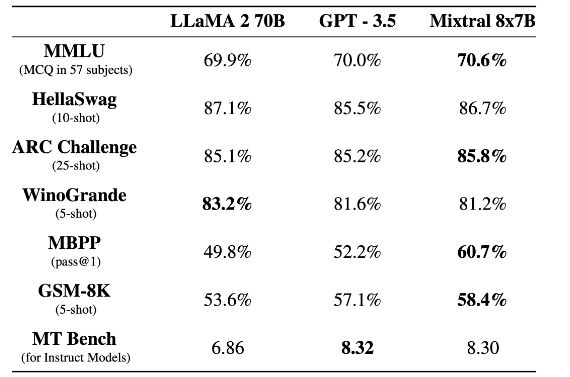
\includegraphics[width=0.75\textwidth,keepaspectratio]{imaxes/5_TablaComparativa.png}
  \caption[Tabla comparativa de modelos]{Tabla comparativa de modelos. \textit{Fuente: \cite{MixtralWebOficial}}}
  \label{fig:5_TablaComparativa}
\end{figure}
``

\section{Alternativa al Fine-Tuning: RAG}

Los sistemas que utilizan \acrshort{RAG} (ver la sección \ref{subsubsec:enfoquerag}), al incorporar fuentes externas de información, se facilita a los modelos generar respuestas más precisas y relevantes. De esta manera, no se requiere volver a entrenar el modelo; en su lugar, se utiliza la información contextual proporcionada durante la generación para ofrecer una respuesta mejorada.

\bigskip % Deja una línea en blanco

En este instante es cuando un sistema \acrshort{RAG} entra en acción. Cuando un usuario hace una búsqueda, el sistema encuentra los documentos internos más importantes y los incluye en la búsqueda al \acrshort{LLMs}. Este tipo de consulta mejorada ayuda al \acrshort{LLMs} a generar respuestas más precisas y educadas, evitando la necesidad de entrenar de nuevo. Asimismo, la posibilidad del sistema de mencionar la fuente en la que se fundamenta su respuesta aumenta la confianza de los usuarios al proporcionar un mayor nivel de fiabilidad.

\bigskip % Deja una línea en blanco

En primer lugar, es necesario transferir la información a nuestro sistema, la cual puede consistir en documentos de texto de diversos tipos y formatos (PDFs de artículos de investigación, HTML de páginas web, archivos en Markdown de una Wiki interna, tickets en un sistema de organización de trabajo, etc.). Hemos decidido usar el archivo de datos \acrshort{JSON} en nuestro sistema, el cual ya ha sido utilizado previamente en diversas secciones para entrenar distintos modelos.

\bigskip % Deja una línea en blanco

En esta etapa, optamos por dividir el texto en fragmentos, también llamados \textit{chunks}, separando así los documentos extensos en secciones más manejables. Esto es importante porque los \textit{\gls{embeddings}} tienen capacidad limitada para representar significado en forma vectorial. Al incluir y organizar estos fragmentos más pequeños en lugar de documentos completos, el sistema puede encontrar y obtener de manera más precisa las secciones más importantes para las consultas de los usuarios. En nuestra iniciativa, hemos procedido de la manera siguiente.

\bigskip % Deja una línea en blanco

\begin{lstlisting}[language=Python, caption={Fragmentación de texto.}, label=listado11]
from langchain.text_splitter import CharacterTextSplitter

text_splitter = CharacterTextSplitter(
    chunk_size=7500, chunk_overlap=100
)
doc_splits = text_splitter.split_documents(docs_list)

# Verificar el contenido de los splits
for split in doc_splits:
    print(split.page_content, split.metadata)

\end{lstlisting}

\bigskip % Deja una línea en blanco

La división de texto asegura que la información importante esté bien organizada al crear el \textit{prompt} para el modelo generativo.

\bigskip % Deja una línea en blanco

Alcanzado este punto, es necesario iniciar la búsqueda; por lo tanto, es crucial comprender el funcionamiento de los \gls{embeddings}. Cada palabra, frase, párrafo, o documento de cierta longitud se asigna a un vector numérico en un espacio de representación donde el texto se considera 'embebido'.

\bigskip % Deja una línea en blanco

\begin{figure}[htbp!]
  \centering
  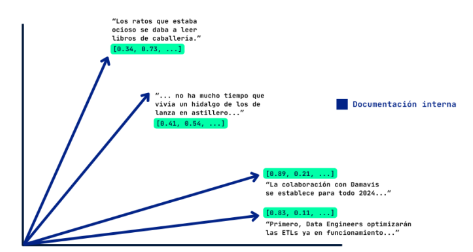
\includegraphics[width=\textwidth,keepaspectratio]{imaxes/5_RAG_Embeddingpng.png}
  \caption[Esquema vectorial del modelo embedding]{Esquema vectorial del modelo embedding. \textit{Fuente: \cite{embedding}}}
  \label{fig:5_RAG_Embedding}
\end{figure}


\bigskip % Deja una línea en blanco

El modelo de \textit{embedding} será adecuado si textos semánticamente relacionados se asignan a vectores que sean cercanos \ref{fig:5_RAG_Embedding}. Estos textos salen fragmentados con una longitud fija, la cual pasarán a llamarse nodos, donde posteriormente, a partir de un modelo \textit{embedding} y el nodo, se calculan los vectores. Donde posteriormente pasarán a almacenarse en bases de datos especialmente diseñadas para vectores de gran cantidad de componentes, que los guardan haciendo una gestión eficiente de la memoria y permitiendo, a través de distintas técnicas de indexado, mejorar la eficiencia de la búsqueda de vectores vecinos.

\bigskip % Deja una línea en blanco

En el caso que estamos estudiando, decidimos emplear el modelo de \textit{embedding} de código libre \textbf{nomic-embed-text-v1} \cite{Nomic}, el cual nos brinda acceso a una \acrshort{API} gratuita de 1 millón de tokens. En su lugar, podríamos haber optado por utilizar diferentes \textit{embeddings} más distintivos, como los de OpenAI, como por ejemplo text-embedding-ada-002, que tiene un costo asociado. Además, elegimos \textbf{ChromaDB} \cite{Chroma} como base de datos vectorial debido a su potencia y versatilidad para manejar y consultar \textit{embeddings}, mejorando las capacidades de búsqueda semántica y recuperación de datos en aplicaciones avanzadas de inteligencia artificial. En la figura \ref{fig:5_RAG_Esquema} se presenta un esquema de la configuración del procedimiento que estamos ejecutando.

\bigskip % Deja una línea en blanco

\begin{figure}[htbp!]
  \centering
  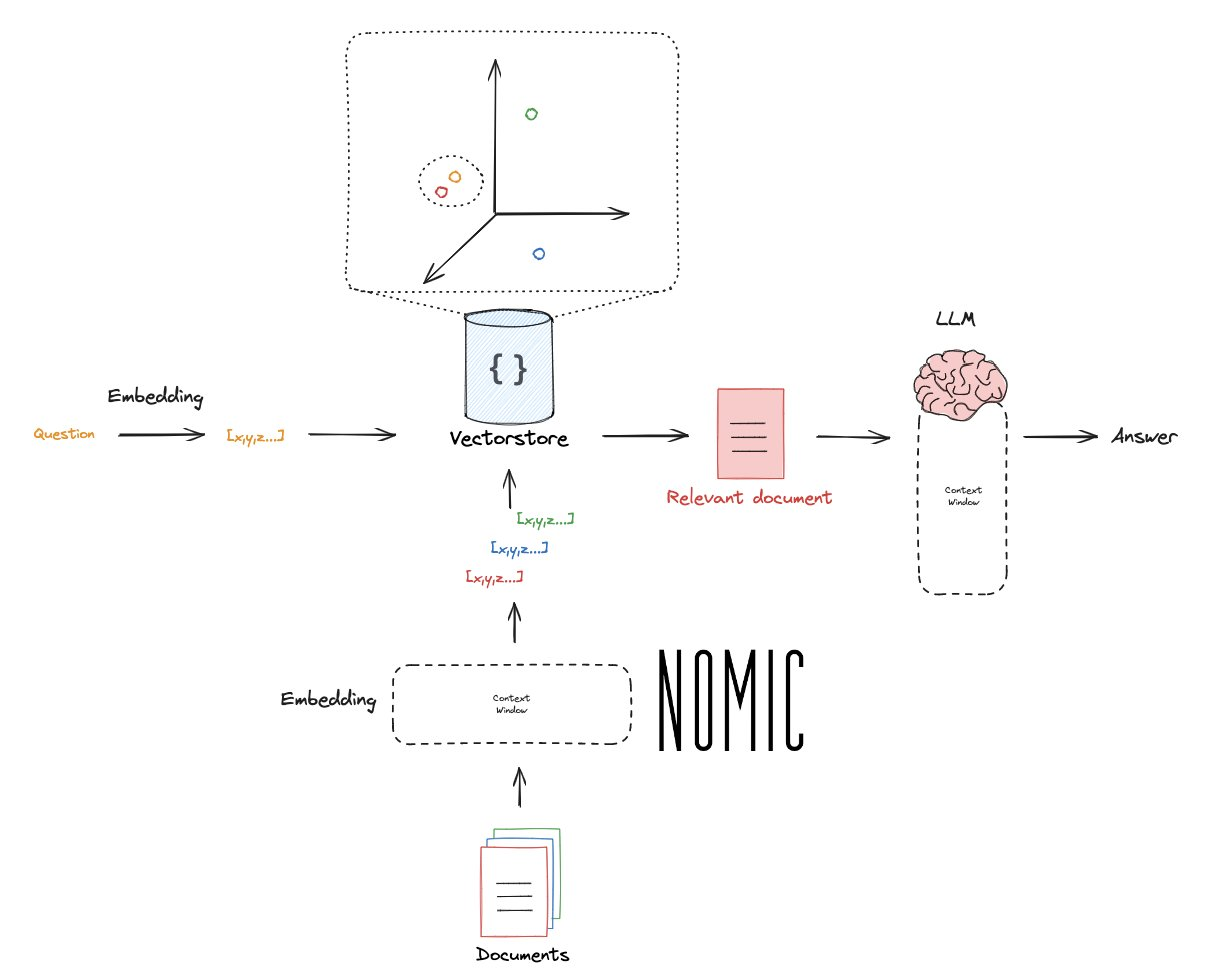
\includegraphics[width=0.85\textwidth,keepaspectratio]{imaxes/5_RAG_Esquema.jpeg}
  \caption[Esquema del proceso RAG]{Esquema del proceso RAG. \textit{Fuente: \cite{LangChainAI2023}}}
  \label{fig:5_RAG_Esquema}
\end{figure}


\bigskip % Deja una línea en blanco

En esta etapa, nos situamos en la fase de generación, en la cual podremos crear una respuesta basada en los \textit{prompts} incluidos en el archivo de entrada. Usaremos el mismo modelo que hemos estado utilizando en esta investigación, que es el \textbf{gpt-3.5-turbo} de OpenAI. Indudablemente, uno de los modelos más idóneos para satisfacer las características de nuestro proyecto.

\bigskip % Deja una línea en blanco

Al igual que hicimos con el enfoque Fine-Tuning, hemos optado por llevar a cabo un conjunto de métricas en el proceso para evaluar la eficacia de este sistema \acrshort{RAG} en nuestra iniciativa. Las métricas utilizadas son las mismas que se mencionaron anteriormente (subsección \ref{subsec:evaluaciónmodelos}), por lo que podemos tener una idea general de los resultados anticipados.

\bigskip % Deja una línea en blanco

\begin{table}[ht!]
  \centering
  \scalebox{0.90}{ % Cambia el valor 0.90 para ajustar el tamaño
    \rowcolors{2}{white}{gray!25}
    \begin{tabular}{c|c|c|c|c}
      \rowcolor{pink!25}
      \textbf{Modelos} & \textbf{Precisión} & \textbf{Recall} & \textbf{F1 Score} & \textbf{\acrshort{BLEU}} \\\hline
      RAG - Modelo GPT & 0.909& 0.909 & 0.909 & 0.032 \\
    \end{tabular}
  }
  \caption{Tabla resultados de métricas de GPT con RAG.}
  \label{tab:TablaMetricas}
\end{table}

\bigskip % Deja una línea en blanco

Basándonos en los resultados previos presentados \ref{tab:TablaMetricas}, podemos inferir las siguientes conclusiones:

\bigskip % Deja una línea en blanco

\begin{itemize}
    \item \textbf{Precisión (Precision)}: El 90.9\% de las predicciones positivas hechas por el modelo fueron precisas. Esto señala que el modelo es bastante preciso y tiene una tasa baja de falsos positivos.
    \item \textbf{Recuperación (Recall):} El 90.9\% de las instancias realmente positivas fueron identificadas correctamente por el modelo. Esto indica que el modelo puede recuperar la mayor parte de los casos importantes, presentando una tasa baja de falsos negativos.
    \item \textbf{Puntuación F1 (F1 Score):} El F1 Score representa la combinación armónica de la precisión y el recall, siendo en este caso 0.909. Esto señala un balance apropiado entre precisión y recall, lo cual es deseado en una tarea donde ambas métricas tienen la misma importancia.
    \item \textbf{\acrfull{BLEU}:} En comparación con las otras métricas, la puntuación BLEU es notablemente inferior. Un score de 0.032 indica que, a pesar de la precisión y el buen recall del modelo para identificar las categorías correctas, la generación de texto puede no coincidir de forma efectiva con el texto de referencia en términos de fluidez y coherencia.
\end{itemize}

\bigskip % Deja una línea en blanco

El rendimiento del modelo \acrshort{RAG} con \acrshort{GPT}-3.5 Turbo en términos de precisión y recall es extraordinario, logrando un 90.9\% en ambos aspectos, lo que demuestra su eficacia en la identificación y clasificación precisa de elementos relevantes. No obstante, el bajo puntuaje \acrshort{BLEU} de 0.032 indica que la calidad del texto producido requiere mejoras para aumentar su coherencia y naturalidad, subrayando la necesidad de optimizar la generación de respuestas a fin de mejorar la fluidez y concordancia con las referencias humanas.

\bigskip % Deja una línea en blanco

Al igual que en proyectos anteriores, y por nuestro compromiso con el desarrollo de código abierto, documentaremos todo el proceso y lo subiremos a Hugging Face en el enlace mencionado. (\href{https://huggingface.co/eibeel/gpt_RAG_TFG}{Enlace}).

\bigskip % Deja una línea en blanco

Después de examinar Fine-Tuning y \acrshort{RAG}, podemos concluir y comparar los dos modelos.

\bigskip % Deja una línea en blanco

El \textbf{Fine-Tuning} mejora la precisión y la consistencia de respuestas al optimizar modelos para tareas específicas, reduciendo además la latencia de inferencia. Sin embargo, el proceso es costoso y lento debido a la necesidad de volver a entrenar para actualizar los datos, y puede carecer de flexibilidad al estar adaptado para ciertos sectores.

\bigskip % Deja una línea en blanco


En contraste, el método \textbf{\acrshort{RAG}} facilita la inclusión de datos recientes sin requerir otro entrenamiento del sistema, disminuyendo gastos y tiempos de actualización, y brindando respuestas exactas con base en documentos pertinentes. No obstante, se necesita infraestructura extra para recuperar documentos, está basado en la calidad del corpus y puede causar demoras en las respuestas.

\bigskip % Deja una línea en blanco

Tras analizar los distintos aspectos, podemos concluir que el enfoque \acrshort{RAG} ofrece soluciones excelentes para nuestro problema, con un coste y dificultad de proceso considerablemente menores que el Fine-Tuning, según se menciona en el artículo de investigación \cite{ovadia2024finetuning}. Sin embargo, esta no es una solución universal ya que estará determinada por las particularidades y necesidades de cada proyecto \ref{fig:5_RAG_RAGvsFineTuning}.

\bigskip % Deja una línea en blanco

\begin{figure}[htbp!]
  \centering
  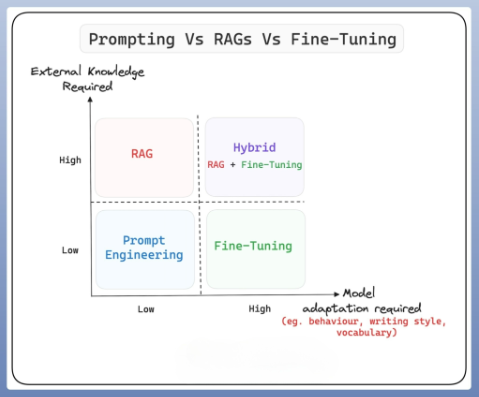
\includegraphics[width=0.85\textwidth,keepaspectratio]{imaxes/5_RAG_RAGvsFineTuning.png}
  \caption[Comparativa RAG vs Fine-Tuning]{Comparativa RAG vs Fine-Tuning. \textit{Fuente: \cite{Celik2023}}}
  \label{fig:5_RAG_RAGvsFineTuning}
\end{figure}



 \chapter{Seguridad, Ética y Aspectos Legales}
\label{chap:etica}

\lettrine{E}{}n el campo de la generación automática de código mediante modelos de lenguaje masivos, emergen preocupaciones importantes que van más allá del rendimiento técnico y abarcan aspectos de seguridad, ética y cumplimiento legal.

En este capítulo, se examinan detalladamente los temas esenciales, proporcionando un análisis exhaustivo sobre las consideraciones de seguridad necesarias para proteger sistemas y datos, así como los dilemas éticos relacionados con el uso de la inteligencia artificial y las regulaciones legales que rigen estas tecnologías avanzadas.

El propósito es orientar el desarrollo y la implementación de herramientas de generación de código que sean no solo efectivas, sino también responsables y seguras.


\section{Consideraciones de Seguridad}

La implementación de modelos de lenguaje masivos en la generación de código conlleva desafíos de seguridad que exigen una gestión meticulosa para prevenir errores y ataques que comprometan la integridad del software y los datos.

\begin{itemize}
    \item \textbf{Seguridad del Software Generado}: La calidad del código generado por los modelos de lenguaje puede variar, y sin la supervisión adecuada, algunos pueden introducir vulnerabilidades. Es crucial implementar revisiones de código y pruebas automatizadas para identificar y mitigar posibles riesgos de seguridad en el código producido.
    
    \item \textbf{Seguridad de Datos}: Los datos utilizados y generados por los modelos de lenguaje deben estar protegidos contra accesos no autorizados y manipulaciones. Implementar cifrado de datos y asegurar canales de comunicación son pasos esenciales para proteger la información sensible.
    
    \item \textbf{Robustez del Modelo}: Es vital asegurar que los modelos sean resistentes a ataques adversarios, especialmente en entornos donde actores maliciosos pueden intentar inducir respuestas erróneas o manipular el comportamiento del modelo. Técnicas como el \gls{adversaltraining} pueden mejorar la robustez de los modelos frente a tales ataques.
\end{itemize}

\section{Aspectos Éticos y de Privacidad}

El uso de modelos de lenguaje masivos para la generación de código también plantea importantes cuestiones éticas y de privacidad que deben ser consideradas para mantener la confianza y la aceptación del usuario.

\begin{itemize}
    \item \textbf{Transparencia}: Es crucial que tanto desarrolladores como usuarios entiendan el proceso mediante el cual los modelos generan código, permitiéndoles tomar decisiones informadas. Esto requiere que las operaciones y decisiones del modelo se expliquen de forma que sean accesibles y claras para los humanos.

    \item \textbf{Privacidad}: Es fundamental asegurar que los datos personales solo se utilicen con el consentimiento explícito de los individuos, particularmente en contextos donde se manejan grandes volúmenes de datos para el entrenamiento de modelos. Debe existir un marco de políticas de privacidad bien definidas, alineadas con normativas vigentes como el \acrshort{GDPR}\cite{GDPR2023}.
\end{itemize}


\section{Cumplimiento Legal y Normativo}

Los avances en la generación automática de código también deben cumplir con un marco legal y normativo que garantice que la implementación de estas tecnologías se lleve a cabo de manera ética y conforme a la ley.

\begin{itemize}
    \item \textbf{Cumplimiento de \acrshort{GDPR}}: Los modelos de lenguaje utilizados para la generación automática de código deben cumplir con el \acrshort{GDPR}, asegurando la protección adecuada de los datos personales durante el procesamiento. Esto implica adoptar medidas técnicas y organizativas para garantizar la privacidad y seguridad de la información personal utilizada a lo largo de todo el proceso de generación de código.
    
    \item \textbf{Propiedad Intelectual}: La generación de código plantea preguntas sobre la propiedad del código generado y su originalidad. Las empresas y desarrolladores deben navegar por las leyes de derechos de autor para evitar infracciones.
    
    \item \textbf{Estándares y Certificaciones}: El cumplimiento de estándares internacionales y la obtención de certificaciones pertinentes son cruciales para validar la seguridad y fiabilidad de las soluciones de generación de código. Esto facilita su adopción en sectores regulados. Se pueden encontrar ejemplos detallados en el Apéndice \ref{chap:estandares}.

\end{itemize}
 \chapter{Conclusiones}
\label{chap:conclusions}

\lettrine{E}{}l estudio ha demostrado que la implementación de modelos de lenguaje masivos como \acrshort{GPT}, \acrshort{LLaMA}, y Mixtral puede mejorar significativamente la eficiencia en la generación automática de código. Los modelos entrenados han demostrado una capacidad notable para interpretar descripciones en lenguaje natural y generar código funcional correspondiente. A través de técnicas como Fine-Tuning y \acrfull{RAG}, se ha logrado ajustar estos modelos para optimizar su rendimiento y precisión en tareas específicas de generación de código.

\bigskip % Deja una línea en blanco

Los resultados de experimentos muestran que, aunque los modelos de \textbf{Fine-Tuning} son precisos en situaciones específicas, el enfoque \textbf{\acrshort{RAG}} es más flexible al combinar datos de múltiples fuentes, lo que podría mejorar la creatividad y adaptabilidad ante exigencias de programación complicadas. No obstante, se ha notado que también existen desafíos importantes en la gestión de recursos computacionales y en la optimización de estos modelos para tareas específicas, especialmente en cuanto al tiempo de entrenamiento y al uso de recursos.

\bigskip % Deja una línea en blanco

También se ha demostrado que no hay una única respuesta correcta al problema en general, es decir, dependiendo de las necesidades del proyecto, un tipo de enfoque y un modelo específico se adaptarán mejor. Es esencial contar con una comprensión general de los beneficios que ofrece cada tipo de modelo disponible en el mercado.

\bigskip % Deja una línea en blanco

Por último, este estudio busca iniciar una serie de investigaciones en el campo de los \acrshort{LLMs}, ya que las limitaciones de recursos y de tiempo han impedido profundizar en más modelos y abordar cada uno de ellos en mayor detalle.

\newpage
\section{Lecciones aprendidas y relación con la titulación}

La realización de este \acrshort{TFG} me ha permitido introducirme en el mundo de los \acrshort{LLMs} y de la \acrshort{GenAI}, donde, en gran parte, los conocimientos adquiridos en la asignatura de \textbf{Sistemas Inteligentes} me han servido como base para este nuevo mundo. De igual forma, el haber cursado la asignatura de \textbf{Programación Integrativa} me ha facilitado el manejo de \textit{datasets}, así como el uso de librerías como Tensorflow o Pandas para la manipulación de datos y \textit{datasets}.

\bigskip % Deja una línea en blanco

Además, he podido familiarizarme con modelos más allá de \acrshort{GPT} y así poder tener una visión general de esta tecnología tan innovadora que está teniendo tanto auge en este momento.

\bigskip % Deja una línea en blanco

Para adquirir los conocimientos mencionados a lo largo del proyecto, nos hemos enfrentado a diversas dificultades. Destacan la búsqueda del volumen adecuado de datos para entrenar los modelos, dado que nuestras capacidades computacionales y de almacenamiento son limitadas. Además, hemos tenido que asegurar la máxima similitud entre los entornos de prueba ajustando los parámetros de entrenamiento para mantener la coherencia en la investigación y resolver las particularidades de cada modelo a lo largo del proceso de entrenamiento. 

\bigskip % Deja una línea en blanco

En resumen, estos desafíos han enriquecido significativamente el proyecto, proporcionando una base sólida de experiencia y conocimiento en el campo de la \acrfull{GenAI}.

\section{Trabajo futuro}

La investigación llevada a cabo en este \acrfull{TFG} brinda una base sólida para investigaciones futuras sobre la aplicación de modelos de lenguaje masivo en la generación automatizada de código. 

\bigskip % Deja una línea en blanco

Una posible área de investigación futura es mejorar estos modelos para distintos lenguajes de programación. A pesar de los avances notables con Python, probar la flexibilidad y efectividad de estos modelos en otros idiomas, como JavaScript o Java, podría aumentar considerablemente su uso y importancia en diversos campos de la industria del software.

\bigskip % Deja una línea en blanco

Otra zona fundamental para investigaciones futuras es la creación de métricas y recursos para evaluar de forma eficaz la calidad del código producido. Esto no sólo aumentaría la confianza en la utilización de dichos modelos en ambientes de producción, sino también permitiría detectar y corregir falencias en cuanto a la claridad del código, rendimiento y seguridad.

\bigskip % Deja una línea en blanco

Por último, es crucial considerar las ramificaciones éticas y de seguridad que emergen al desarrollar código de manera automática. 

 %%%%%%%%%%%%%%%%%%%%%%%%%%%%%%%%%%%%%%%%
 % Apéndices, glosarios e bibliografía  %
 %%%%%%%%%%%%%%%%%%%%%%%%%%%%%%%%%%%%%%%%

 \appendix
 \appendixpage
 \chapter{Regulaciones en la Generación de Código}
\label{chap:estandares}

\lettrine{E}{}ste apéndice proporciona un resumen detallado de las certificaciones y estándares relevantes para la generación automática de código, enfocándose en cómo cada uno contribuye a asegurar la calidad, la seguridad y el cumplimiento legal de las soluciones desarrolladas.

\section{Estándares de Seguridad y Calidad}
\begin{itemize}
    \item \textbf{ISO/IEC 27001}: Estándar internacional que proporciona un marco para la gestión de la seguridad de la información. Es esencial para proteger los sistemas que soportan la generación automática de código contra amenazas y vulnerabilidades de seguridad. \cite{ISO27001}
    \item \textbf{ISO/IEC 25010}: Define un modelo de calidad para el software que incluye características clave como funcionalidad, fiabilidad, usabilidad y seguridad. Aplicable en la evaluación de la calidad del código generado automáticamente. \cite{ISO25010}
\end{itemize}

\section{Certificaciones de Cumplimiento de Privacidad}
\begin{itemize}
    \item \textbf{Certificación TrustArc}: Asegura que las prácticas de privacidad de una empresa cumplen con estándares internacionales como el \acrshort{GDPR}, garantizando el manejo adecuado de datos personales en aplicaciones de generación de código. \cite{TrustArc2024}
\end{itemize}

\section{Estándares de Desarrollo de Software}
\begin{itemize}
    \item \textbf{CMMI (Capability Maturity Model Integration)}: Modelo de madurez que mejora los procesos de desarrollo de software, asegurando que el software generado sea de alta calidad y desarrollado en un entorno controlado y sistemático. \cite{CMMIInstitute2024}
\end{itemize}

\section{Certificaciones Legales}
\begin{itemize}
    \item \textbf{ISO 31000}: Proporciona directrices para la gestión de riesgos asociados con el uso de tecnologías emergentes como la generación automática de código, ayudando a las organizaciones a identificar y mitigar posibles riesgos. \cite{ISO31000_2024}
\end{itemize}

\section{Estándares Específicos del Sector}
\begin{itemize}
    \item \textbf{PCI DSS}: Necesario para software que maneja transacciones de pago o datos de tarjetas de crédito, protegiendo contra fraudes y mejorando la seguridad en aplicaciones financieras. \cite{PCIDSS2024}
\end{itemize}

Cada uno de estos estándares y certificaciones representan un papel crucial en diferentes aspectos del desarrollo y despliegue de tecnologías de generación de código, desde la seguridad hasta el cumplimiento legal y la gestión de riesgos.



%\include{anexos/...}

 \printglossary[type=\acronymtype,title=\nomeglosarioacronimos]
 \printglossary[title=\nomeglosariotermos]

 \bibliographystyle{IEEEtranN}
 \bibliography{\bibconfig,bibliografia/bibliografia}
 \clearpage
 
\end{document}

%%%%%%%%%%%%%%%%%%%%%%%%%%%%%%%%%%%%%%%%%%%%%%%%%%%%%%%%%%%%%%%%%%%%%%%%%%%%%%%%
